\documentclass[
    NAME={Dr. Helga Ingimundardóttir},
    EMAIL={helgaingim@hi.is},
    FACULTY={Industrial Engineering},
    TITLE={HiDef Textiles: Reviving Tradition with Innovation},
    SUBTITLE={Empowering Creativity and Sustainability in Textile Production through Digital Transformation},
    SEMINAR={Reykjavík DataBeers},
    DATE={January 25, 2025},
    WIDE={true}
]{HI-LaTeX/hi-beamer}
\usepackage{multimedia,media9}
\usepackage{tikz}
\usepackage{svg}
\usetikzlibrary{positioning, arrows, shapes, fit}
\usepackage{textcomp}


\newcommand{\customframe}[3][]{
    \usebackgroundtemplate{
        \tikz[overlay,remember picture]
        \node[opacity=0.3, at=(current page.center)] {
            \includegraphics[width=\paperwidth,height=\paperheight]{#2}
        };
    }
    \ifx
        &#1&
        \section{#3}
    \fi
    \addtobeamertemplate{frametitle}{\vskip5cm}{} % Adjust the frametitle position for this slide only
    \begin{frame}[plain]{#3}
    #1
    \end{frame}
    \addtobeamertemplate{frametitle}{\vskip-5cm}{} % Reset the frametitle template to default
    \usebackgroundtemplate{}  % Reset the background for the following frames
}

\begin{document}

    \begin{frame}{About the Project}

        \begin{block}{The HiDef Textiles Project}
            This project made STEAM\footnote{S: Science, T: Technology, E: Engineering, A: Arts, M: Mathematics.} fields accessible through innovation in textiles by combining artistic creativity and sustainability. The interdisciplinary collaboration involved the \alert{University of Iceland}, the \alert{Iceland University of the Arts}, and domestic companies and institutions.
        \end{block}

        \begin{itemize}
            \item \textbf{90s Knitting Machine:} Transformed for modern users. The renewal process was used to teach technical literacy innovatively.
            \item \textbf{Objective:} Preserved traditions and brought them into a digital context.
            \item \textbf{Demonstration Tool:} Created a functional machine showcased locally and ready for further development.
        \end{itemize}

    \end{frame}

    \begin{frame}{Inspiration}

        \begin{columns}
            \begin{column}{0.65\textwidth}
                \begin{alertblock}{\href{https://vimeo.com/58580261}{Knitterstream}}
                    An art performance at the \alert{C2-MTL} conference in 2012, where tweets with the hashtag \alert{\#knitterstream} were knitted for the attending audience.
                \end{alertblock}

                \begin{itemize}
                    \item Same type of knitting machine as my grandmother's.
                    \item Software available on \href{https://github.com/borgstrom/KnitterStream/tree/master}{GitHub}.
                    \item Drafts for improvements made at \href{https://web.archive.org/web/20150918225135/http://wiki.fablab.is/wiki/HiKnitterStream}{FabLab Reykjavík} in 2014.
                    \item Proper research project funded by the \alert{Icelandic Student Innovation Fund} in summer 2024.
                \end{itemize}

            \end{column}
            \begin{column}{0.35\textwidth}
                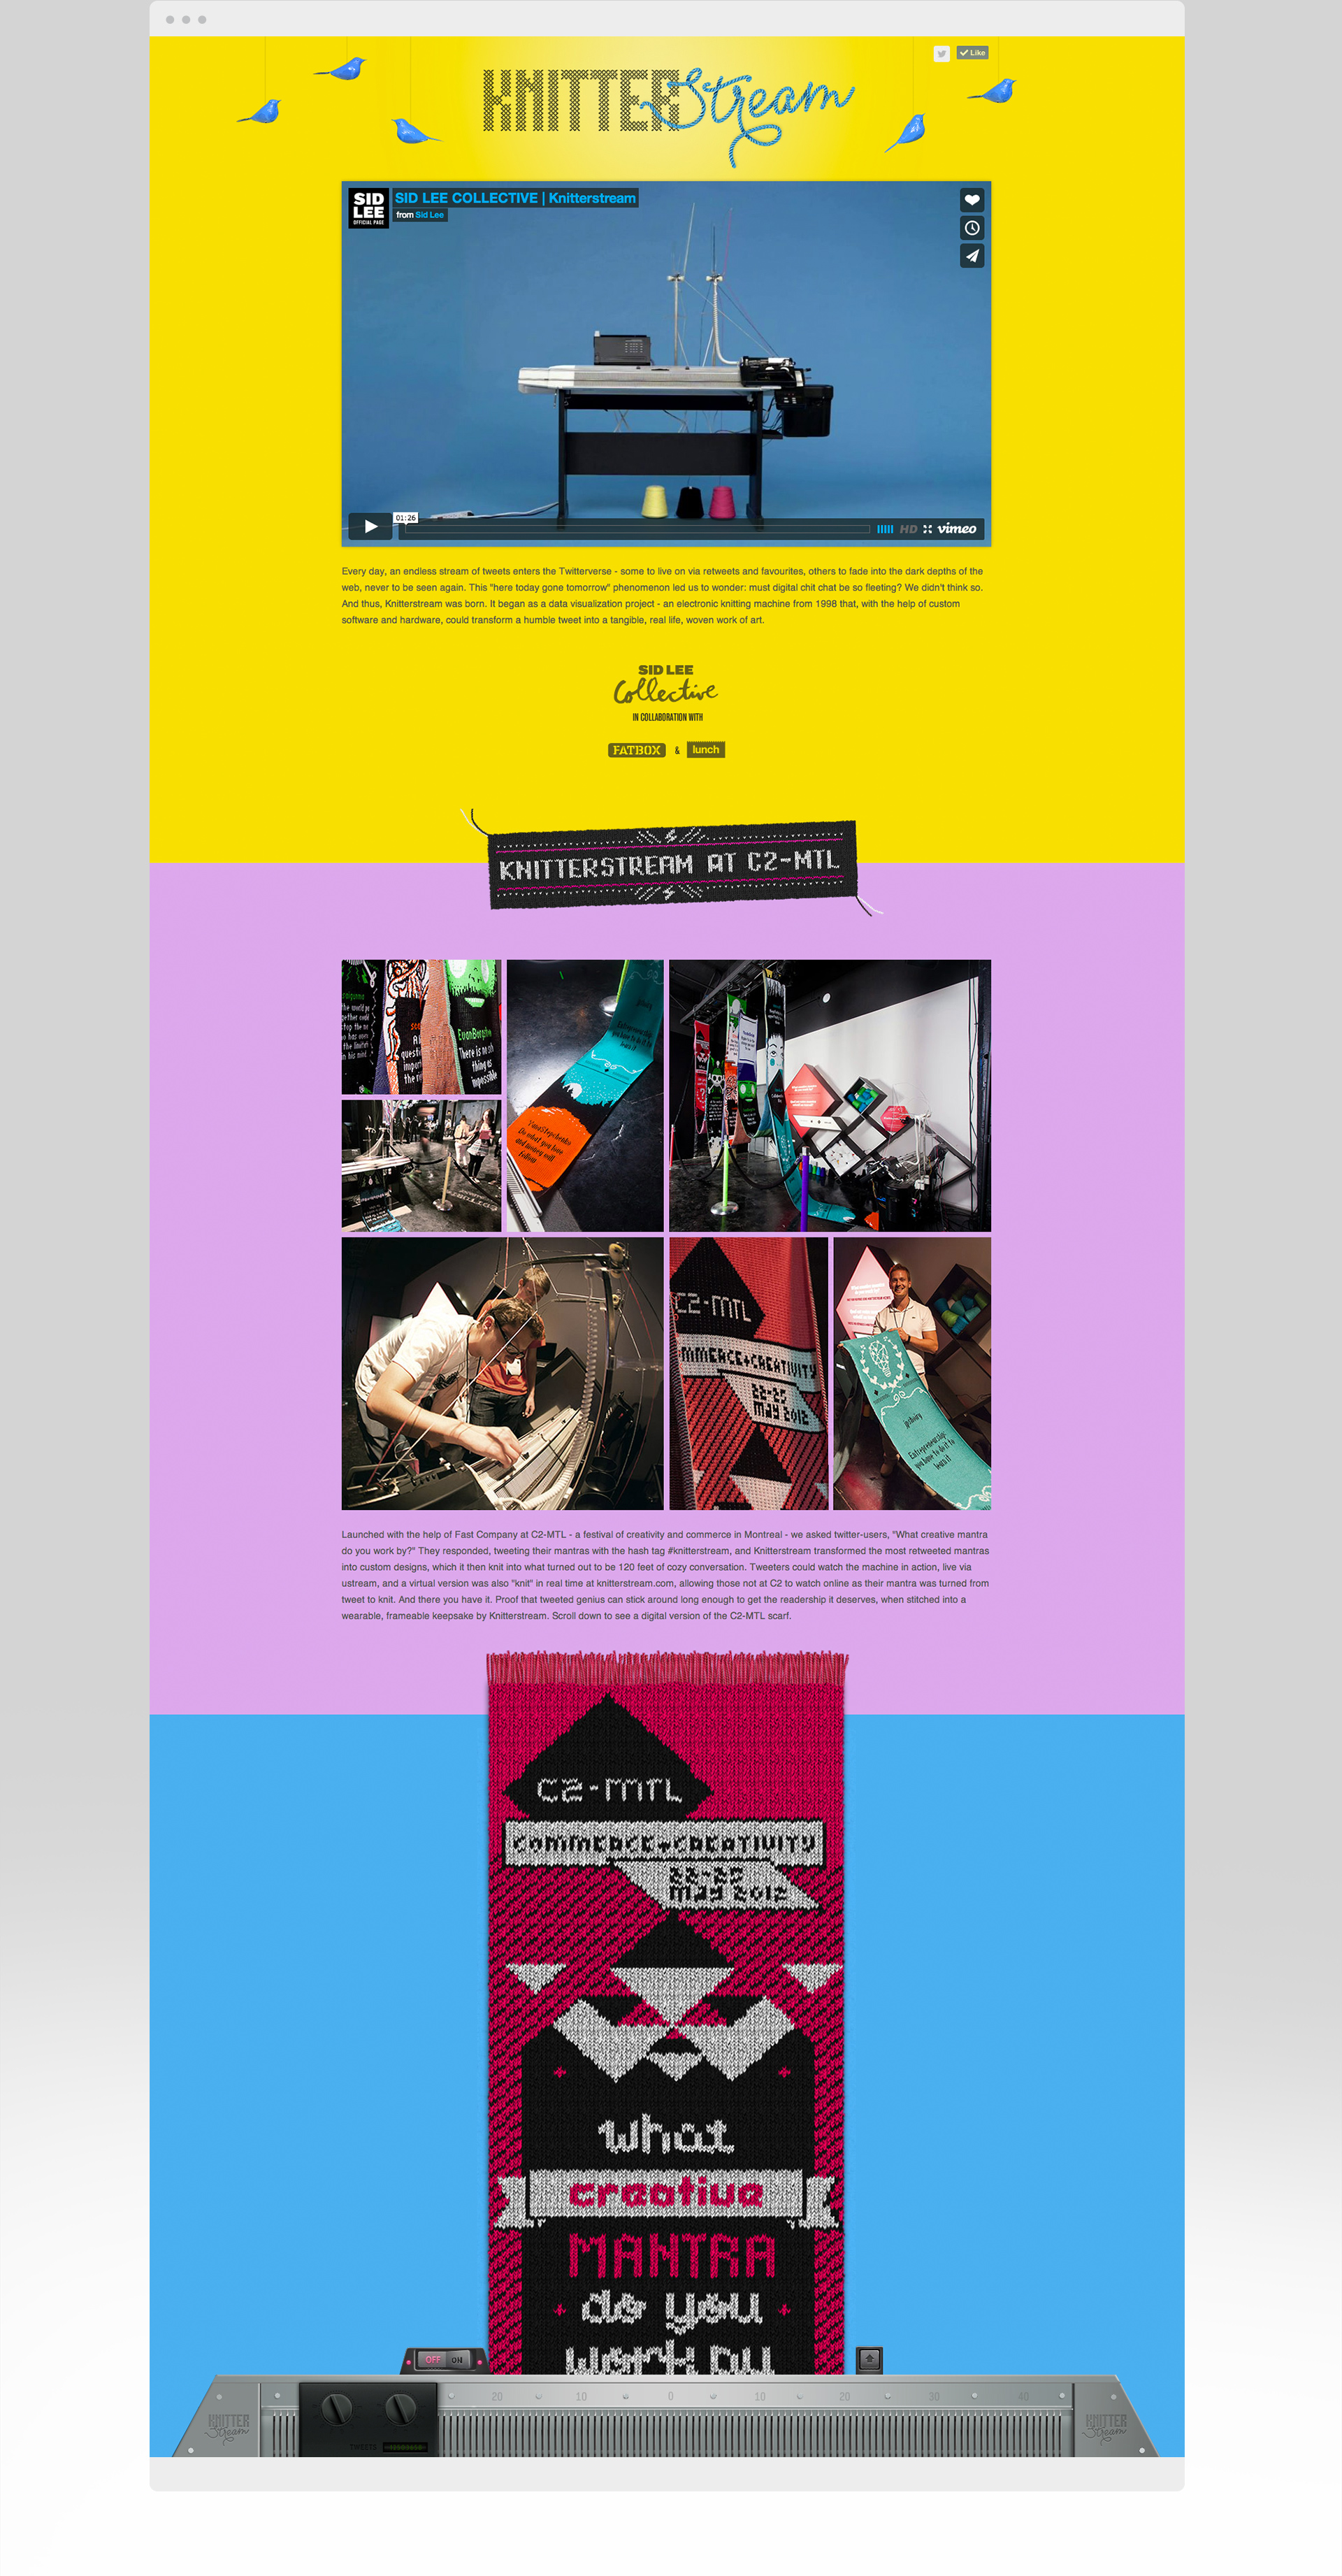
\includegraphics[width=\textwidth, trim={16cm 44cm 16cm 40cm},clip]{include/knitterstream_23.jpg}
            \end{column}

        \end{columns}

    \end{frame}

    \begin{frame}[allowframebreaks]{Participants}
        \begin{columns}
            \begin{column}{0.42\linewidth}
                \begin{block}{Instructors}
                    \begin{description}
                        \item[Hafliði] FABLAB, UI
                        \item[Hafsteinn] Computer Science, UI
                        \item[Helga] Industrial Eng., UI
                        \item[Hörður] Computer \& Electrical Eng., UI
                        \item[Ragna] Fashion Design, IUA
                    \end{description}
                \end{block}
            \end{column}

            \begin{column}{0.45\linewidth}
                \begin{block}{Students}
                    \begin{description}
                        \item[Elli] Mechanical Eng. and Computer Science, UI.
                        \item[Gísa] Fashion Design, IUA.
                        \item[Snæja] Applied Mathematics and Computer Science, UI.
                    \end{description}
                \end{block}
            \end{column}
        \end{columns}

        \framebreak

        \begin{block}{Collaborators}
            \begin{description}
                \item[Icelandic Textile Center] A digital textile workshop in Blöndós, providing spare parts.
                \item[Ístex] Supplies locally sourced yarn.
                \item[The Icelandic Handicraft Association and National Museum of Iceland] Jointly published  \alert{Sjónabók}, which we use as base patterns for our work.
                \item[Marel] A leading manufacturer of equipment for fish processing plants, offering expertise in industrial mechanics and technology.
                \item[\'{Y}rúrarí] \'Yr Jóhannsdóttir, a renowned knitting designer, formerly worked with Passap but now works with \alert{Kniterate}.
                \item[Owen Mace] Retired electrical engineer from South Australia.
            \end{description}
        \end{block}

    \end{frame}

    \customframe[]{include/mbl-e6000.jpg}{Machinery}

    \begin{frame}{Passap Knitting Machines}

% Brief history of Passap
        PASSAP (PAtent Schnell Strick AParat), founded in Switzerland in 1939, was a leader in hobby knitting machines. They ceased production around the turn of the millennium.

% Start the columns environment for comparison
        \begin{columns}

% Left column for Duo 80
            \begin{column}{0.45\textwidth}
                \begin{figure}
                    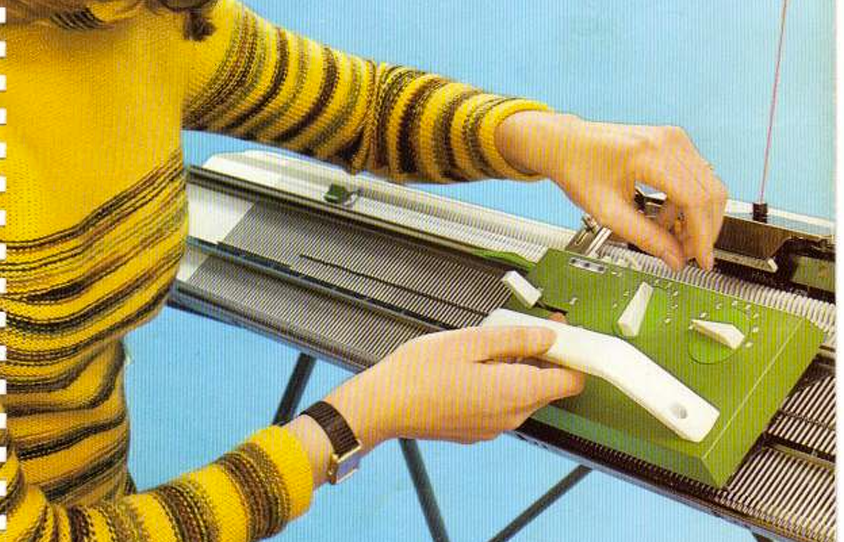
\includegraphics[height=0.3\textheight]{include/duo80.png}
                \end{figure}
                \textbf{Passap Duo 80}
                \begin{itemize}
                    \item \textbf{Motor:} Electra 3000
                    \item \textbf{Color:} Manually switches 4 colors
                    \item \textbf{Pattern:} Simple
                \end{itemize}
            \end{column}

% Right column for E6000
            \begin{column}{0.58\textwidth}
                \begin{figure}
                    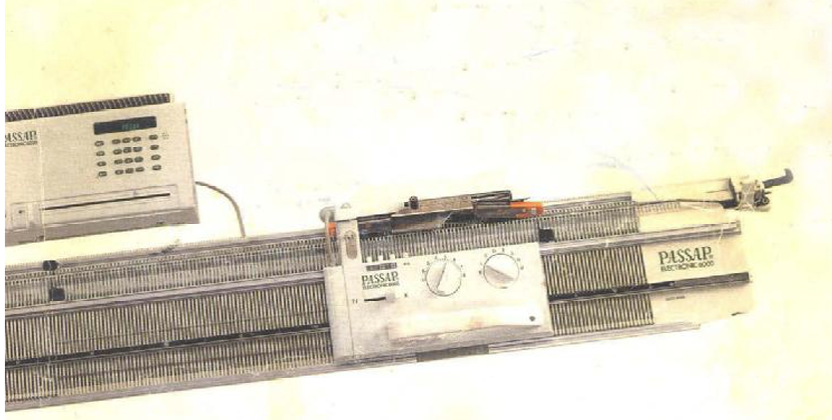
\includegraphics[height=0.3\textheight]{include/e6000.png}
                \end{figure}
                \textbf{Passap E6000}
                \begin{itemize}
                    \item \textbf{Motor:} Electra 4600
                    \item \textbf{Auto Color:} Automatically switches 4 colors
                    \item \textbf{Pattern:} Complex
                \end{itemize}
            \end{column}

        \end{columns}
    \end{frame}

    \begin{frame}{Kniterate}

        \href{https://www.kniterate.com/product/kniterate-the-digital-knitting-machine/}{Kniterate}, a digital knitting machine from Spain, designed for small-batch manufacturers and designers. Only two such machines in Iceland.

        \begin{description}
            \item[Advantage] Originally a ``hack'' of similar 80s/90s knitting machines, it was launched on \href{https://www.kickstarter.com/projects/kniterate/kniterate-the-digital-knitting-machine/}{Kickstarter} in 2017 (then priced at \texteuro{}4,500).
            \item[Disadvantage] Long waiting list and expensive (priced from \texteuro{}16,000).
        \end{description}

        \begin{figure}
            \centering
            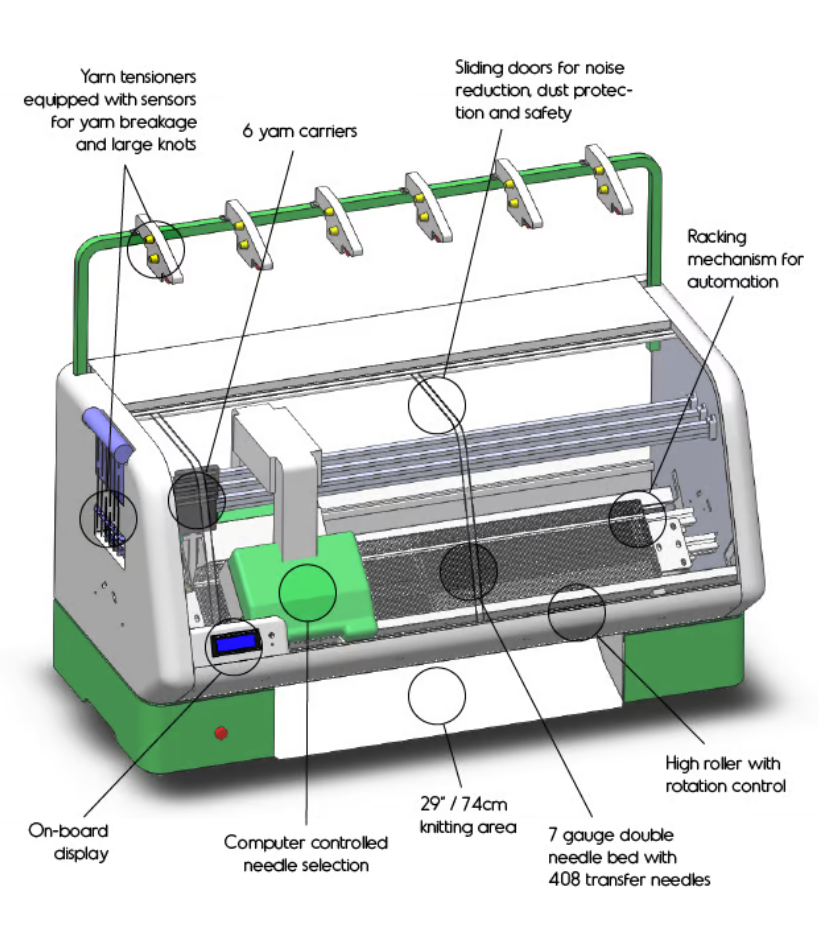
\includegraphics[height=.5\textheight]{include/skema-kniterate.png} ~~~~      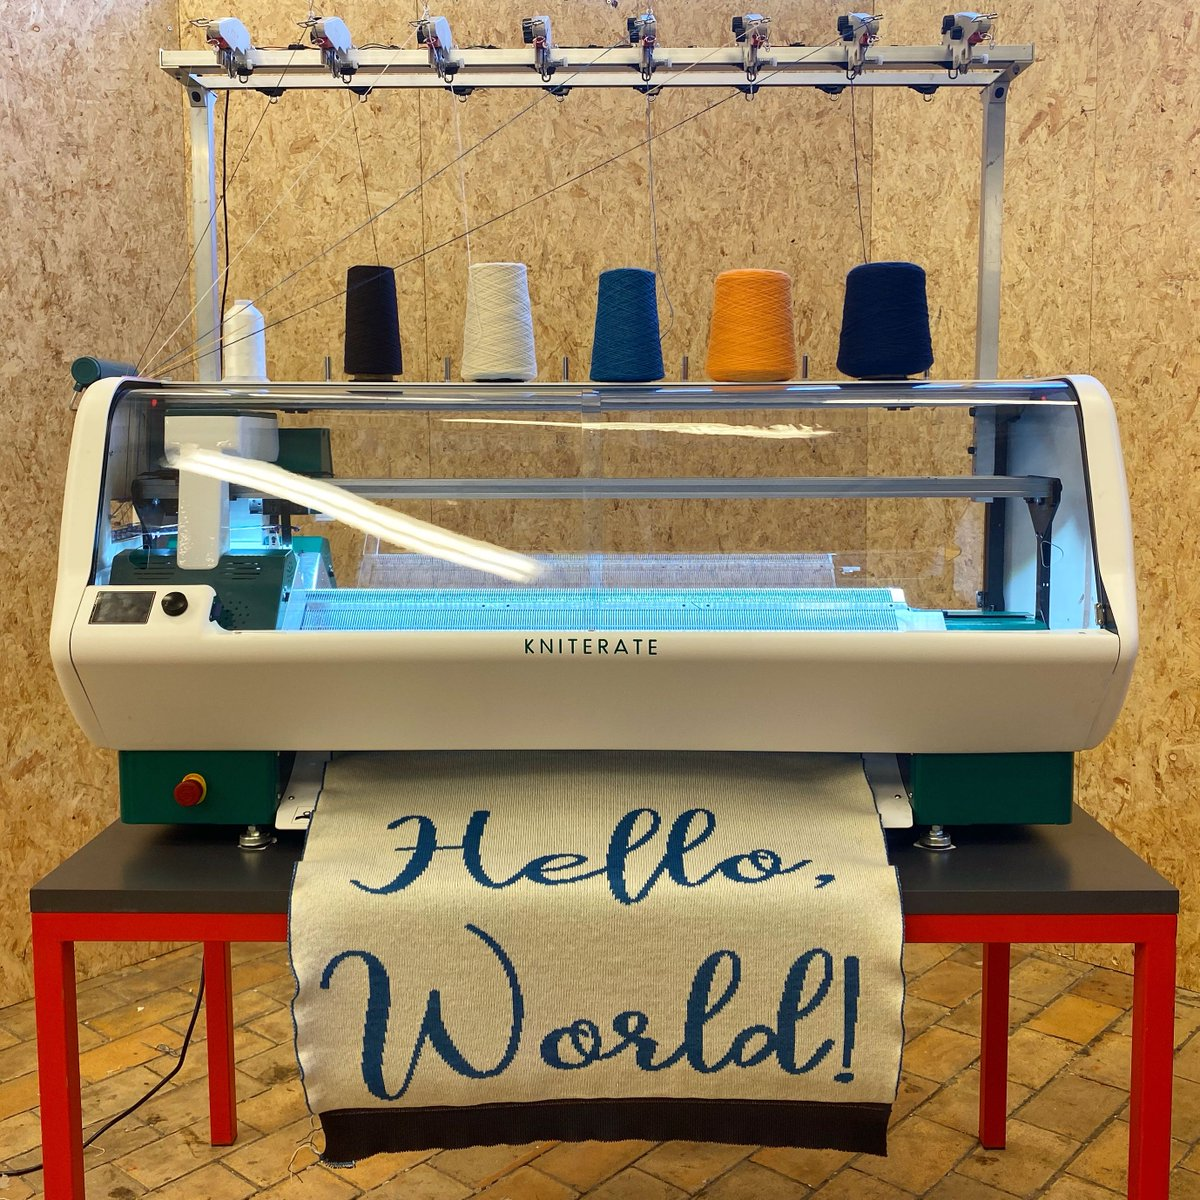
\includegraphics[height=.5\textheight]{include/kniterate-helloworld.jpg}

        \end{figure}
    \end{frame}

    \customframe[]{include/sjónabók-safn.jpg}{Knitting Patterns}

    \begin{frame}[allowframebreaks]{The Icelandic Sjónabók}

        \begin{columns}
            \begin{column}{0.7\textwidth}
                \begin{block}{What is Sjónabók?}
                    It is a culturally significant collection of traditional Icelandic patterns used in various handcrafted items throughout Icelandic history. This manuscript includes patterns from the 16\textsuperscript{th}, 17\textsuperscript{th}, and 18\textsuperscript{th} centuries. Published in 2009, it contains 10 preserved manuscripts and is unfortunately out of print.
                \end{block}

                \begin{itemize}
                    \item \textbf{Translation:} The term ``Sjónabók'' can be translated as ``Book of Visual Patterns.''
                    \item \textbf{Content:} Contains patterns and motifs used in textiles, with text in both Icelandic and English.
                \end{itemize}
            \end{column}

            \begin{column}{0.3\textwidth}
                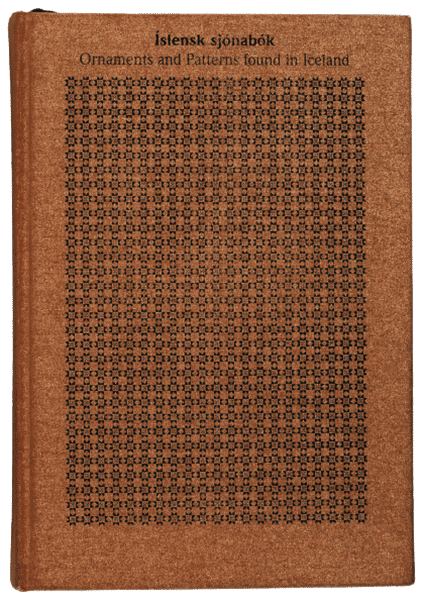
\includegraphics[width=\textwidth]{include/sjónabók.png}
            \end{column}
        \end{columns}

        \framebreak

        \begin{figure}
            \caption{Passage from Hallgrímur Pétursson's  \textit{Passion Hymns}}
            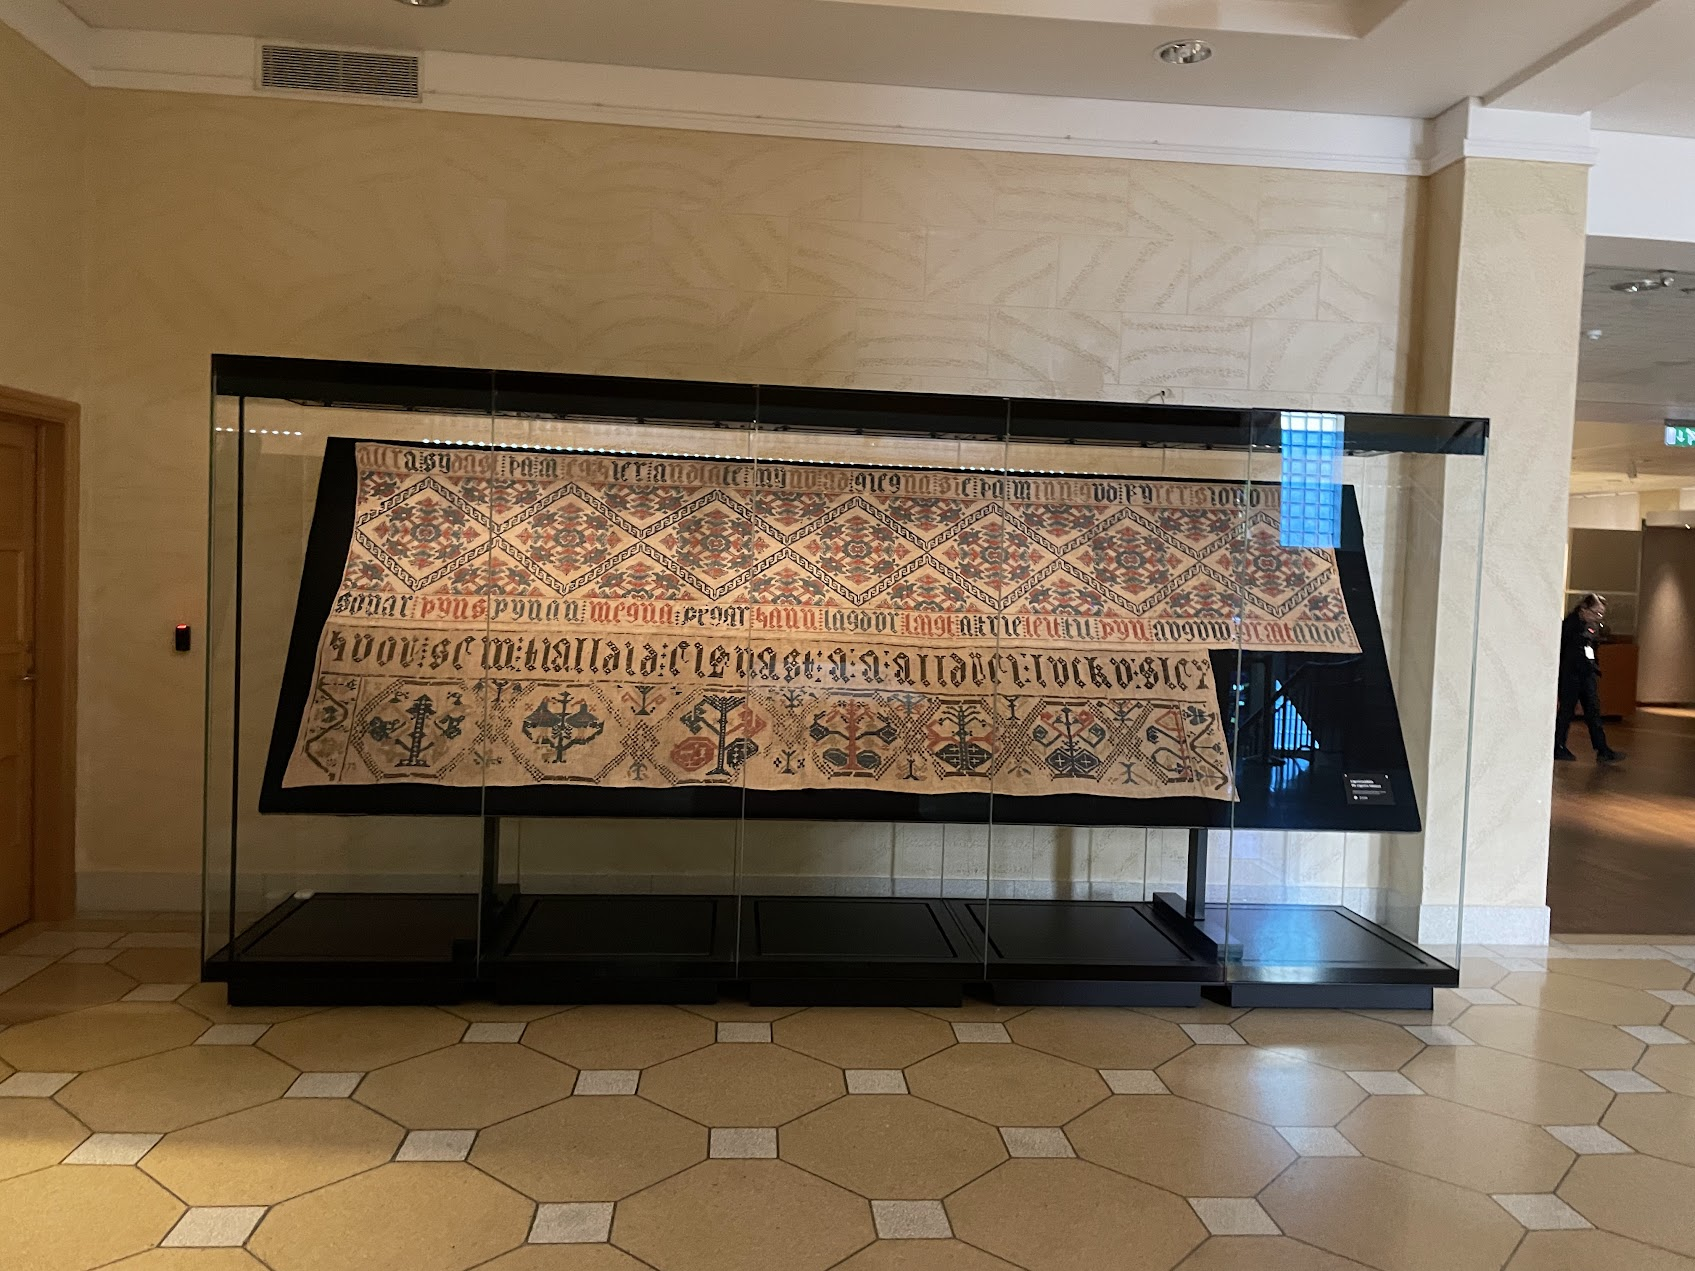
\includegraphics[width=0.49\textwidth]{include/passiusalmur.jpg}
            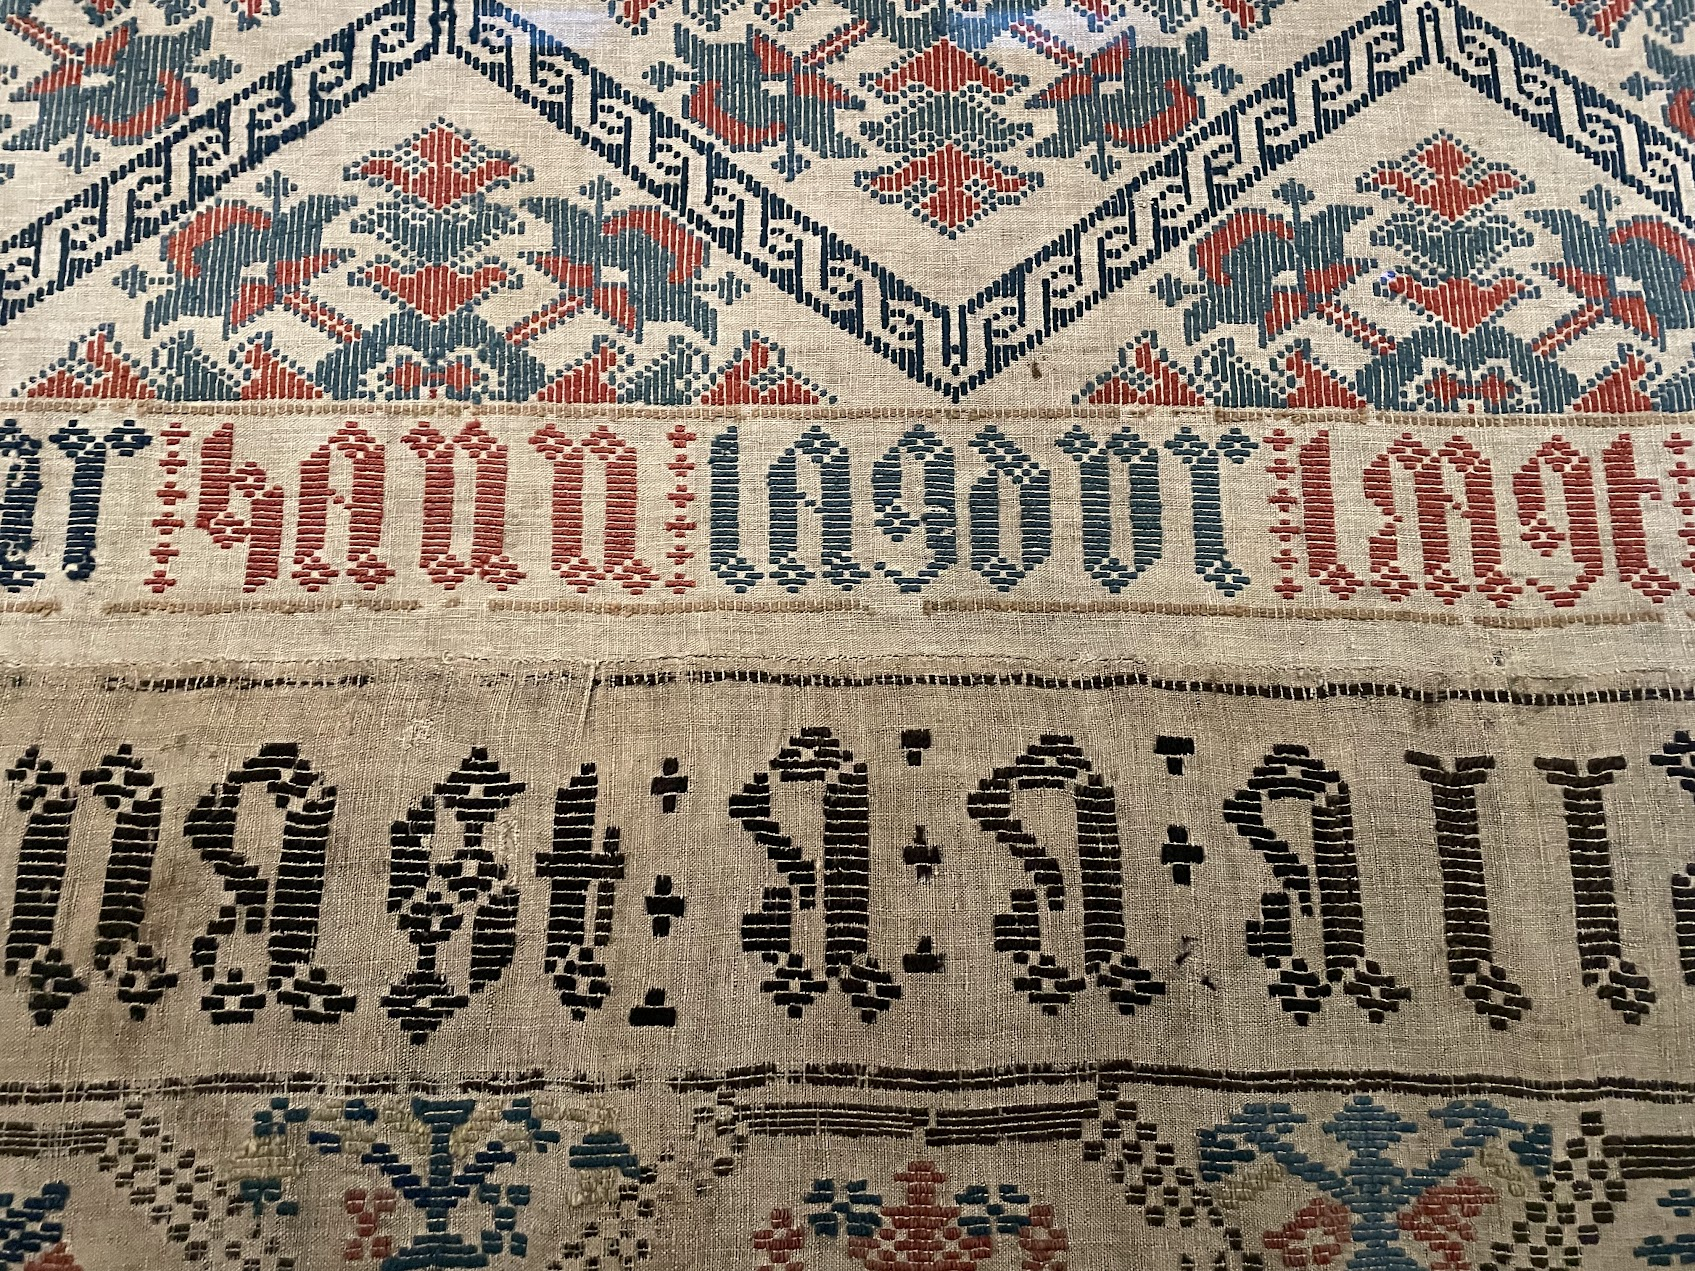
\includegraphics[width=0.49\textwidth]{include/passiusalmur-zoom.jpg}


            \framebreak
            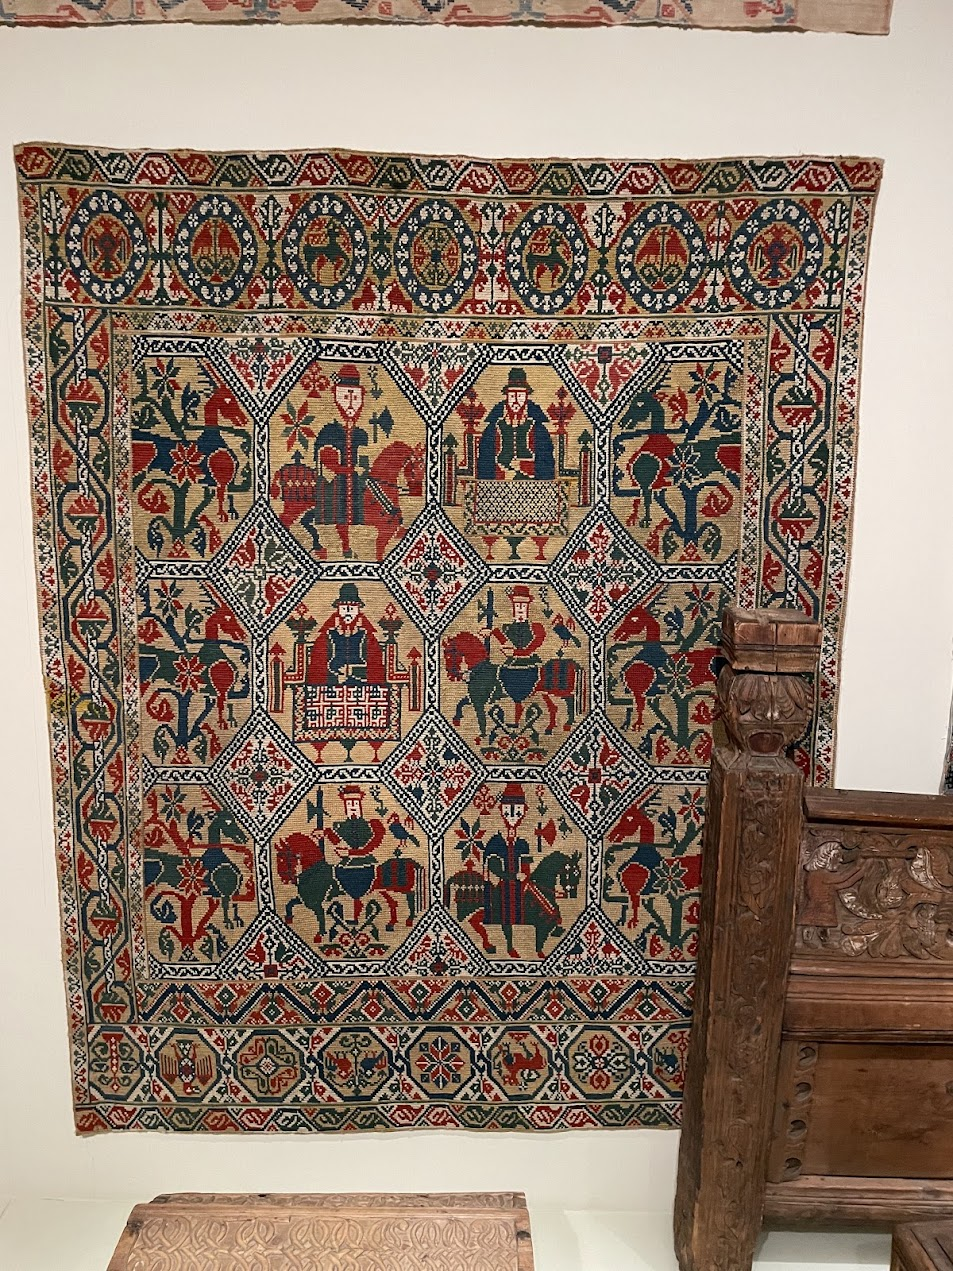
\includegraphics[width=0.3\textwidth]{include/riddarateppi.jpg}
            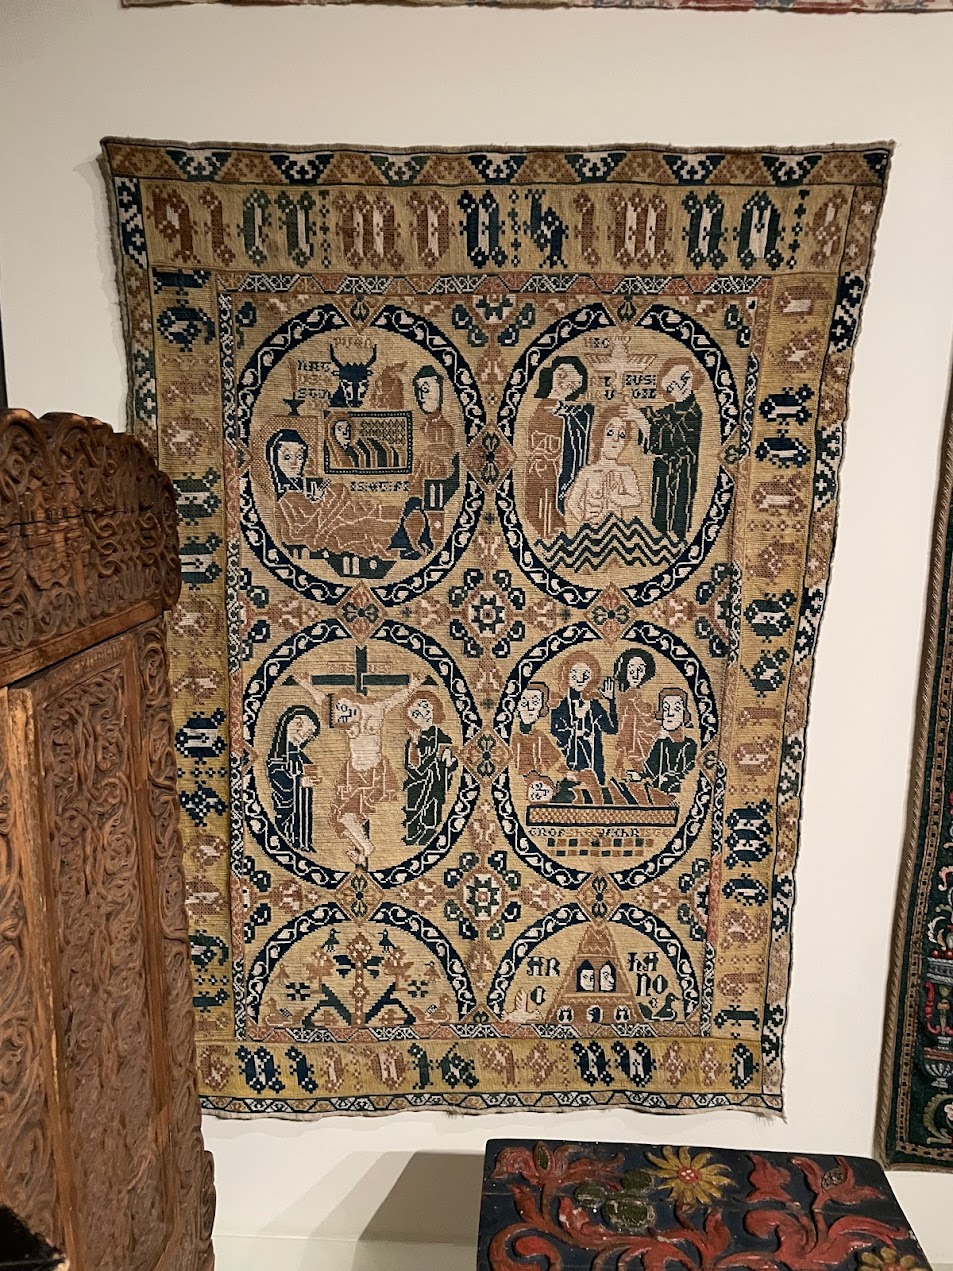
\includegraphics[width=0.3\textwidth]{include/ævijesú.jpg}
        \end{figure}

        \framebreak

        \begin{figure}

            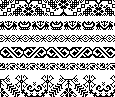
\includegraphics[height=.65\textheight]{include/thjms2008-14_560.png}\hspace{24pt}
            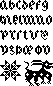
\includegraphics[height=.65\textheight]{include/thjms2008-14_562.png}
        \end{figure}
        \url{https://github.com/HiDefTextiles/Sjonabok}
    \end{frame}

    \customframe[]{include/swatches.jpg}{Knitting Swatches}

    \begin{frame}{Hello World}

        \begin{quote}
            What better way to say we've arrived in the world of digital knitting than...
        \end{quote}

        \begin{figure}
            \centering
            \caption{First try}
            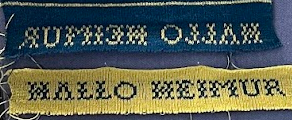
\includegraphics[height=46pt, clip=true, trim=0 5mm 0 0]{include/helloworld.png}

            \caption{Second try (after mirroring)}
            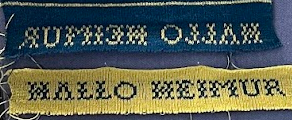
\includegraphics[height=46pt, clip=true, trim=0 0 0 5mm]{include/helloworld.png}
        \end{figure}

    \end{frame}

    \begin{frame}{Icelandic Peacock}
        \centering
        \href{https://www.instagram.com/p/C9Cf8FFgDZZ/}{
            
\includegraphics[height=.7\textheight]{include/thjms5898_246_0.png}
            \hspace{24pt}
            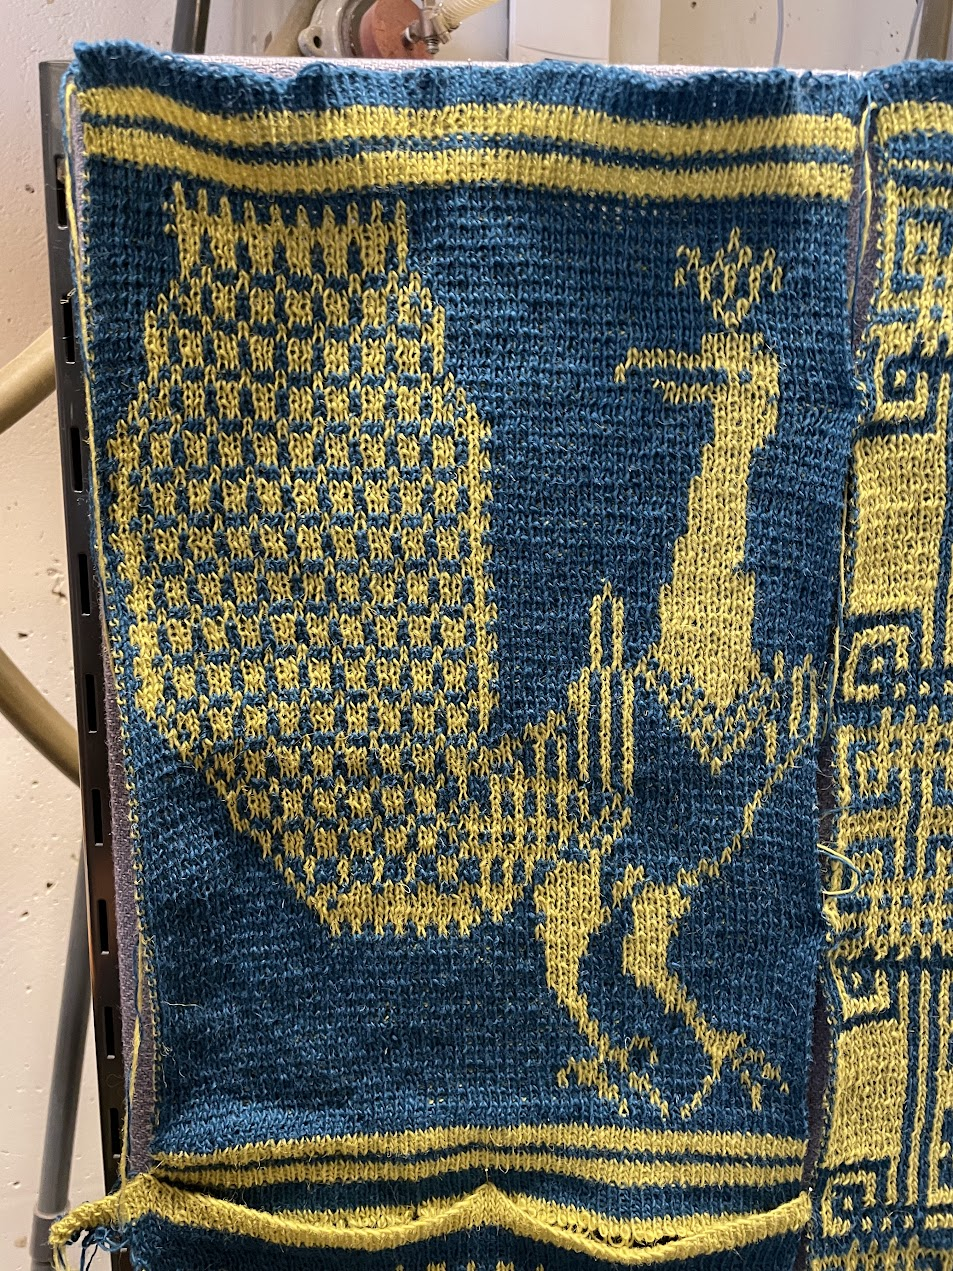
\includegraphics[height=.7\textheight]{include/peacock.jpg}}
    \end{frame}

    \begin{frame}{Icelandic Flower}
        \centering
        
\includegraphics[height=.7\textheight]{include/thjms5898_210.png}
        \hspace{24pt}
        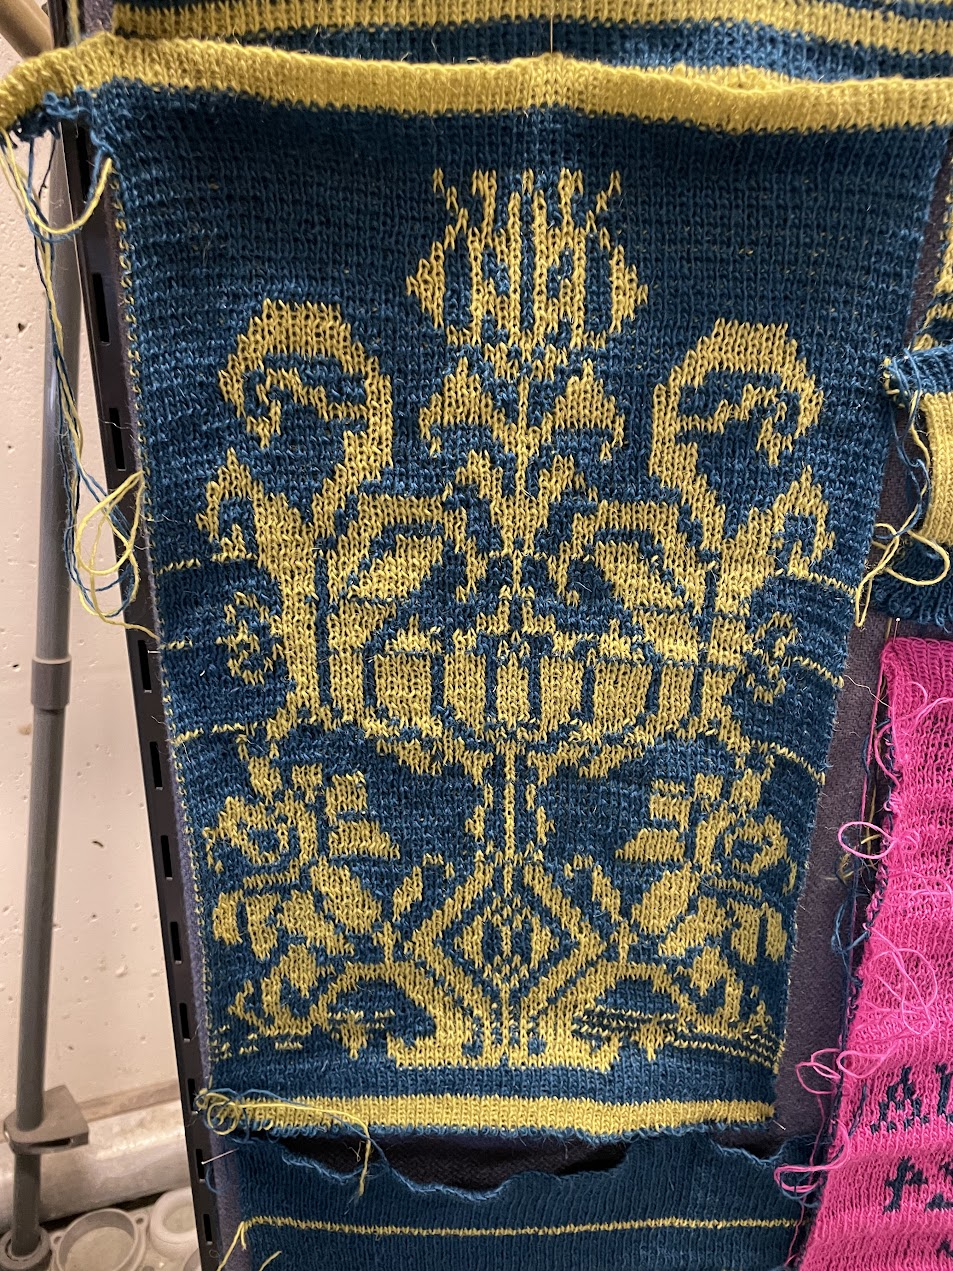
\includegraphics[height=.7\textheight]{include/flower.jpg}
    \end{frame}

    \begin{frame}{Repeated Motif}
        \centering
        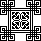
\includegraphics[height=.7\textheight]{include/thjms5898_268.png}
        \hspace{24pt}
        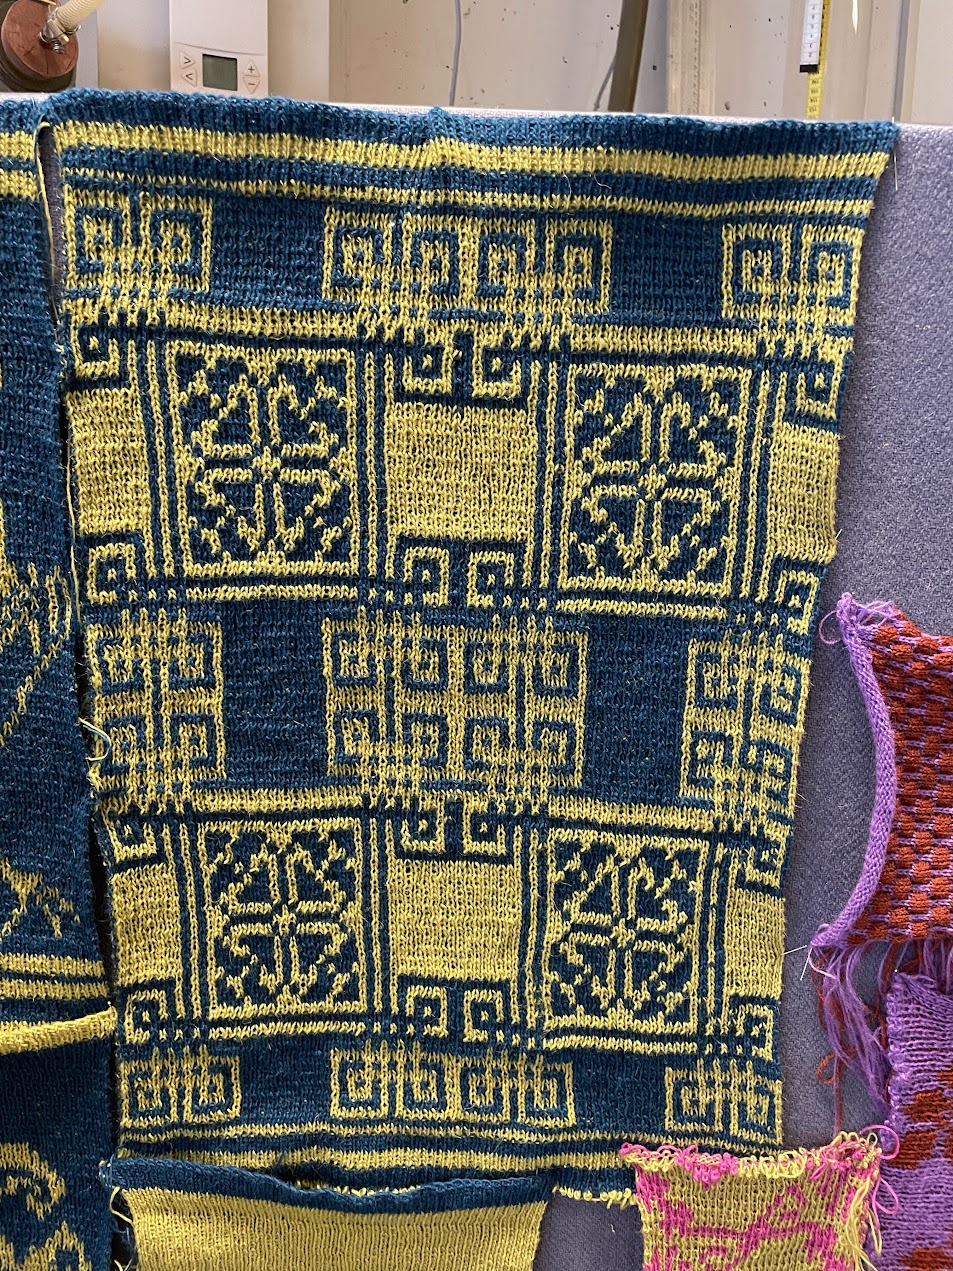
\includegraphics[height=.7\textheight]{include/repeat.jpg}
    \end{frame}


    \begin{frame}{Pets}
        \centering
        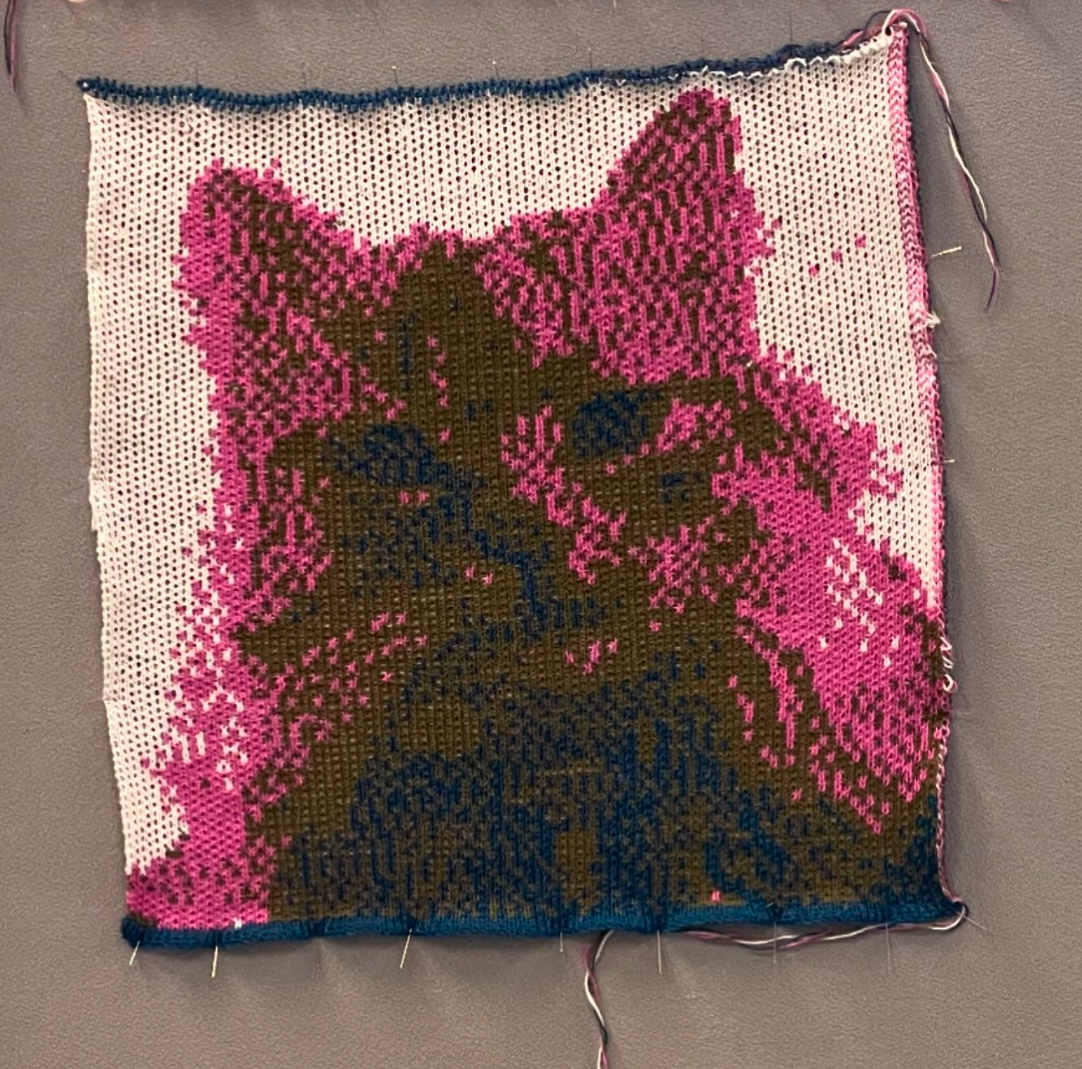
\includegraphics[height=.7\textheight]{include/kisa.png}
        \hspace{24pt}
        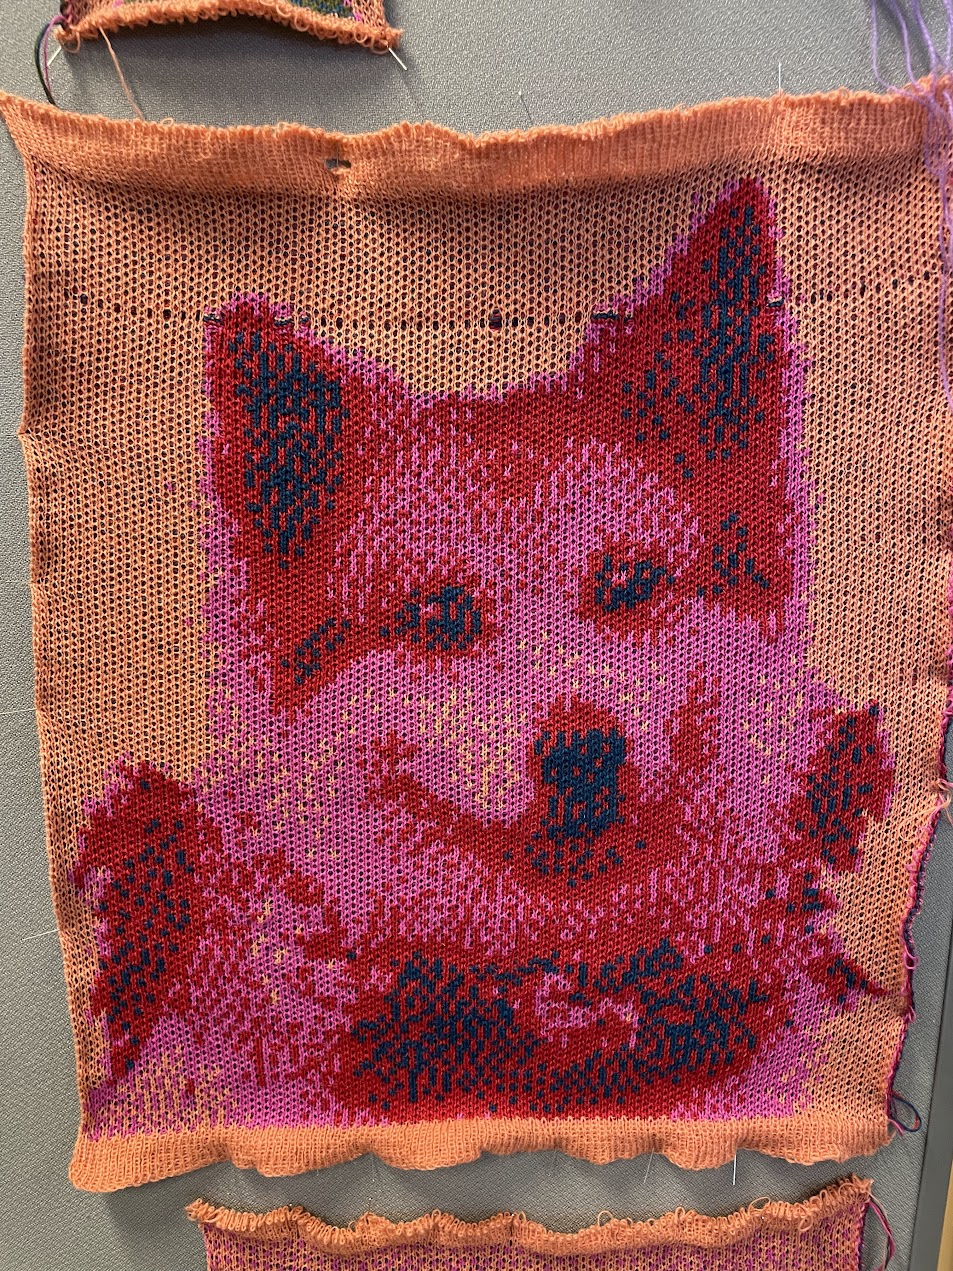
\includegraphics[height=.7\textheight]{include/hundur.jpg}

    \end{frame}


    \begin{frame}{Ragnheiður Jónsdóttir (1646--1715)}
        \begin{columns}
            \begin{column}{.5\linewidth}
                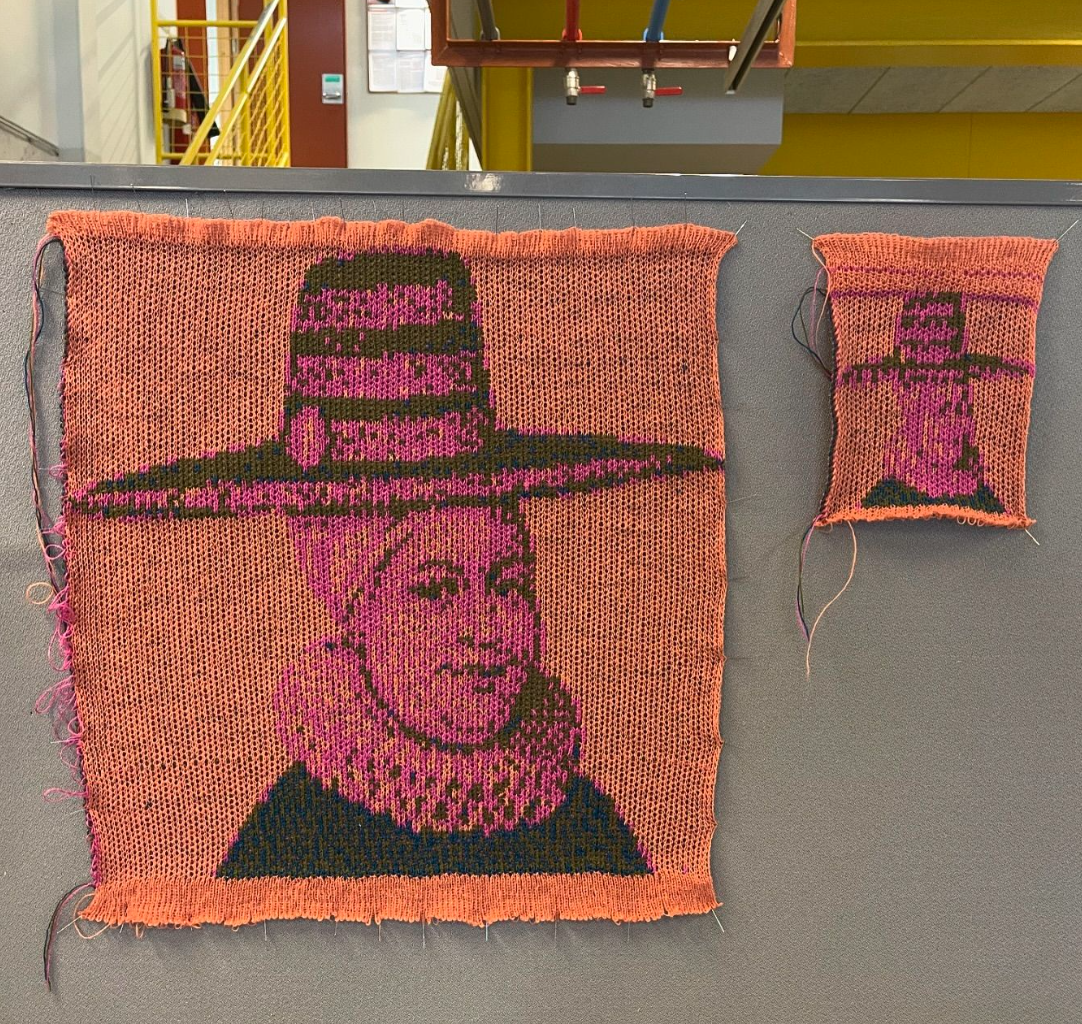
\includegraphics[width=\linewidth]{include/ragnheidur.png}
            \end{column}
            \begin{column}{.5\linewidth}
                \begin{block}{Bishop's Wife}
                    Ragnheiður was a patron of the arts and crafts and played a pivotal role in preserving traditional Icelandic patterns.
                \end{block}
                \centering
                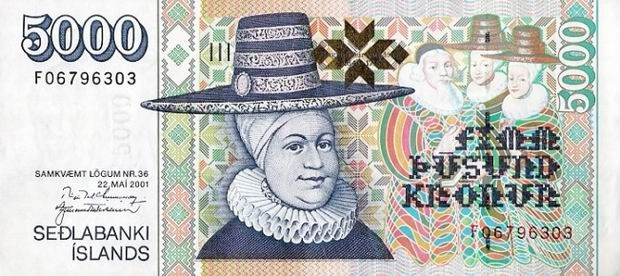
\includegraphics[width=.7\linewidth]{include/5000kr.JPG}
            \end{column}
        \end{columns}
    \end{frame}


    \begin{frame}{Brynjólfur Sveinsson (1605--1675)}
        \begin{columns}
            \begin{column}{.65\linewidth}
                \begin{block}{Bishop of Skálholt}
                    Brynjólfur was the Lutheran Bishop, renowned for his efforts in preserving Icelandic literary heritage. He contributed to the collection of Old Norse manuscripts, including \emph{Book of Flatey}, and played a key role in naming the \emph{Edda} collection.
                \end{block}
                \centering
                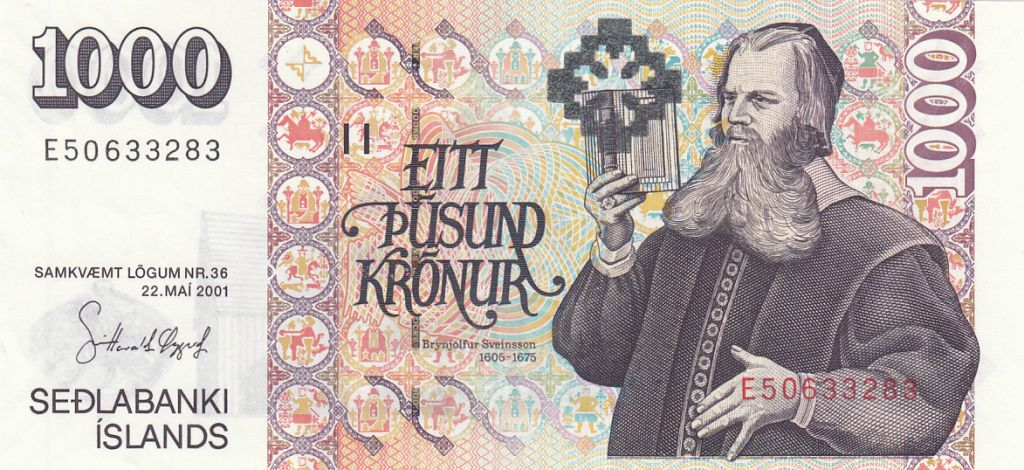
\includegraphics[width=.5\linewidth]{include/1000kr.jpg}
            \end{column}
            \begin{column}{.35\linewidth}
                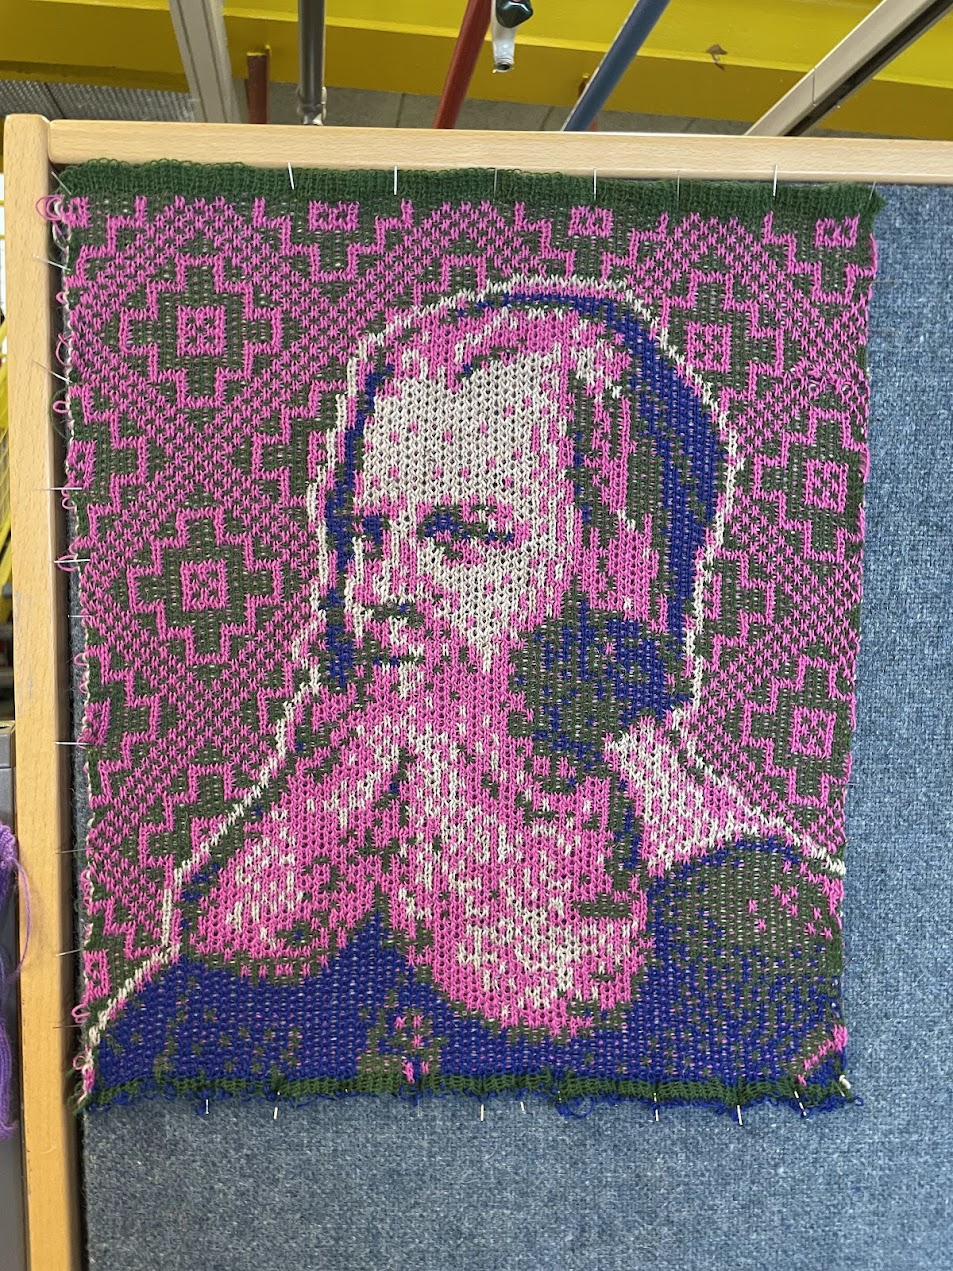
\includegraphics[height=.75\textheight]{include/sveinsson.jpg}
            \end{column}


        \end{columns}

    \end{frame}

    \customframe[]{include/swatches.jpg}{What Next?}

    \begin{frame}{Lessons Learned and Next Steps}
        \begin{itemize}
            \item \textbf{Hardware Improvements:} While the machine is functional, there are kinks in hardware control, especially in color changes, requiring upgrades.
            \item \textbf{Pattern Workflow:} Experimentation with generative AI superimposed with \emph{Sjónabók} patterns shows promise, but the workflow needs further refinement.
            \item \textbf{Future Vision:} Hardware upgrades to make the more common Duo 80 model as capable as the E6000 would be a significant advancement.
        \end{itemize}
    \end{frame}

    \begin{frame}{Generative Patterns}
        \begin{figure}
            \centering
            \begin{tikzpicture}[
                node distance=6pt and 2cm,
                arrow/.style={-stealth, thick},
                image/.style={inner sep=0pt},
                label/.style={font=\small}
            ]
                % Nodes for images
                \node[image] (sjonabok) at (0,0) {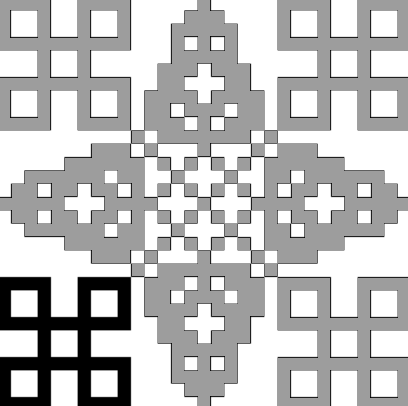
\includegraphics[width=0.1\linewidth]{include/sjonabok_after.png}};
                \node[image, right=of sjonabok] (wfc) {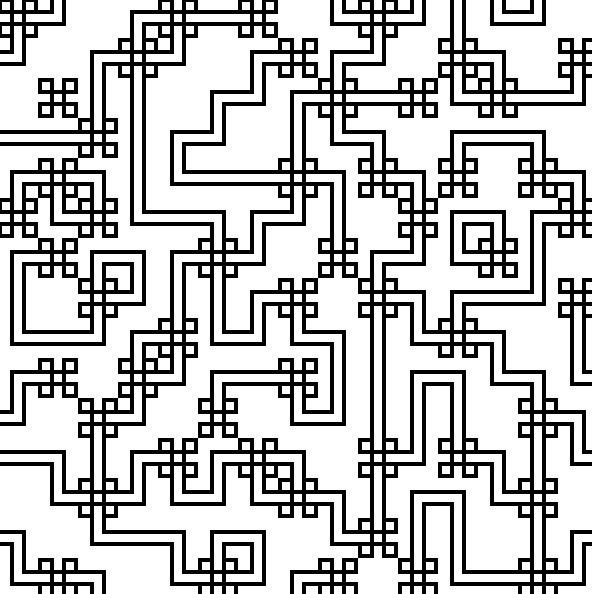
\includegraphics[width=0.3\linewidth]{include/wfc.png}};

                % Labels for the images
                \node[label, below=of sjonabok] {Pattern Source};
                \node[label, below=of wfc] {Generated Pattern};

                % Arrow connecting the images
                \draw[arrow] ([xshift=5mm]sjonabok.east) -- ([xshift=-5mm]wfc.west) node[above, midway, font=\small] {WFC};
            \end{tikzpicture}
            \caption{Preliminary experiments using generative algorithms, like \alert{Wave Function Collapse} (WFC), to create novel patterns inspired by traditional \alert{Sjónabók} motifs.}
        \end{figure}
    \end{frame}


    \begin{frame}{Where Can You See the Machine in Action?}
        \begin{itemize}
            \item \textbf{2024:} \includesvg[height=18pt]{include/logo-visindavaka.svg}
            \item \textbf{2025:}
            \includesvg[height=18pt]{include/logo-utmessan.svg}
            \item \textbf{2026:} Planned for \alert{Design March} and a summer residency at \alert{The Museum of Design and Applied Art}.
        \end{itemize}
        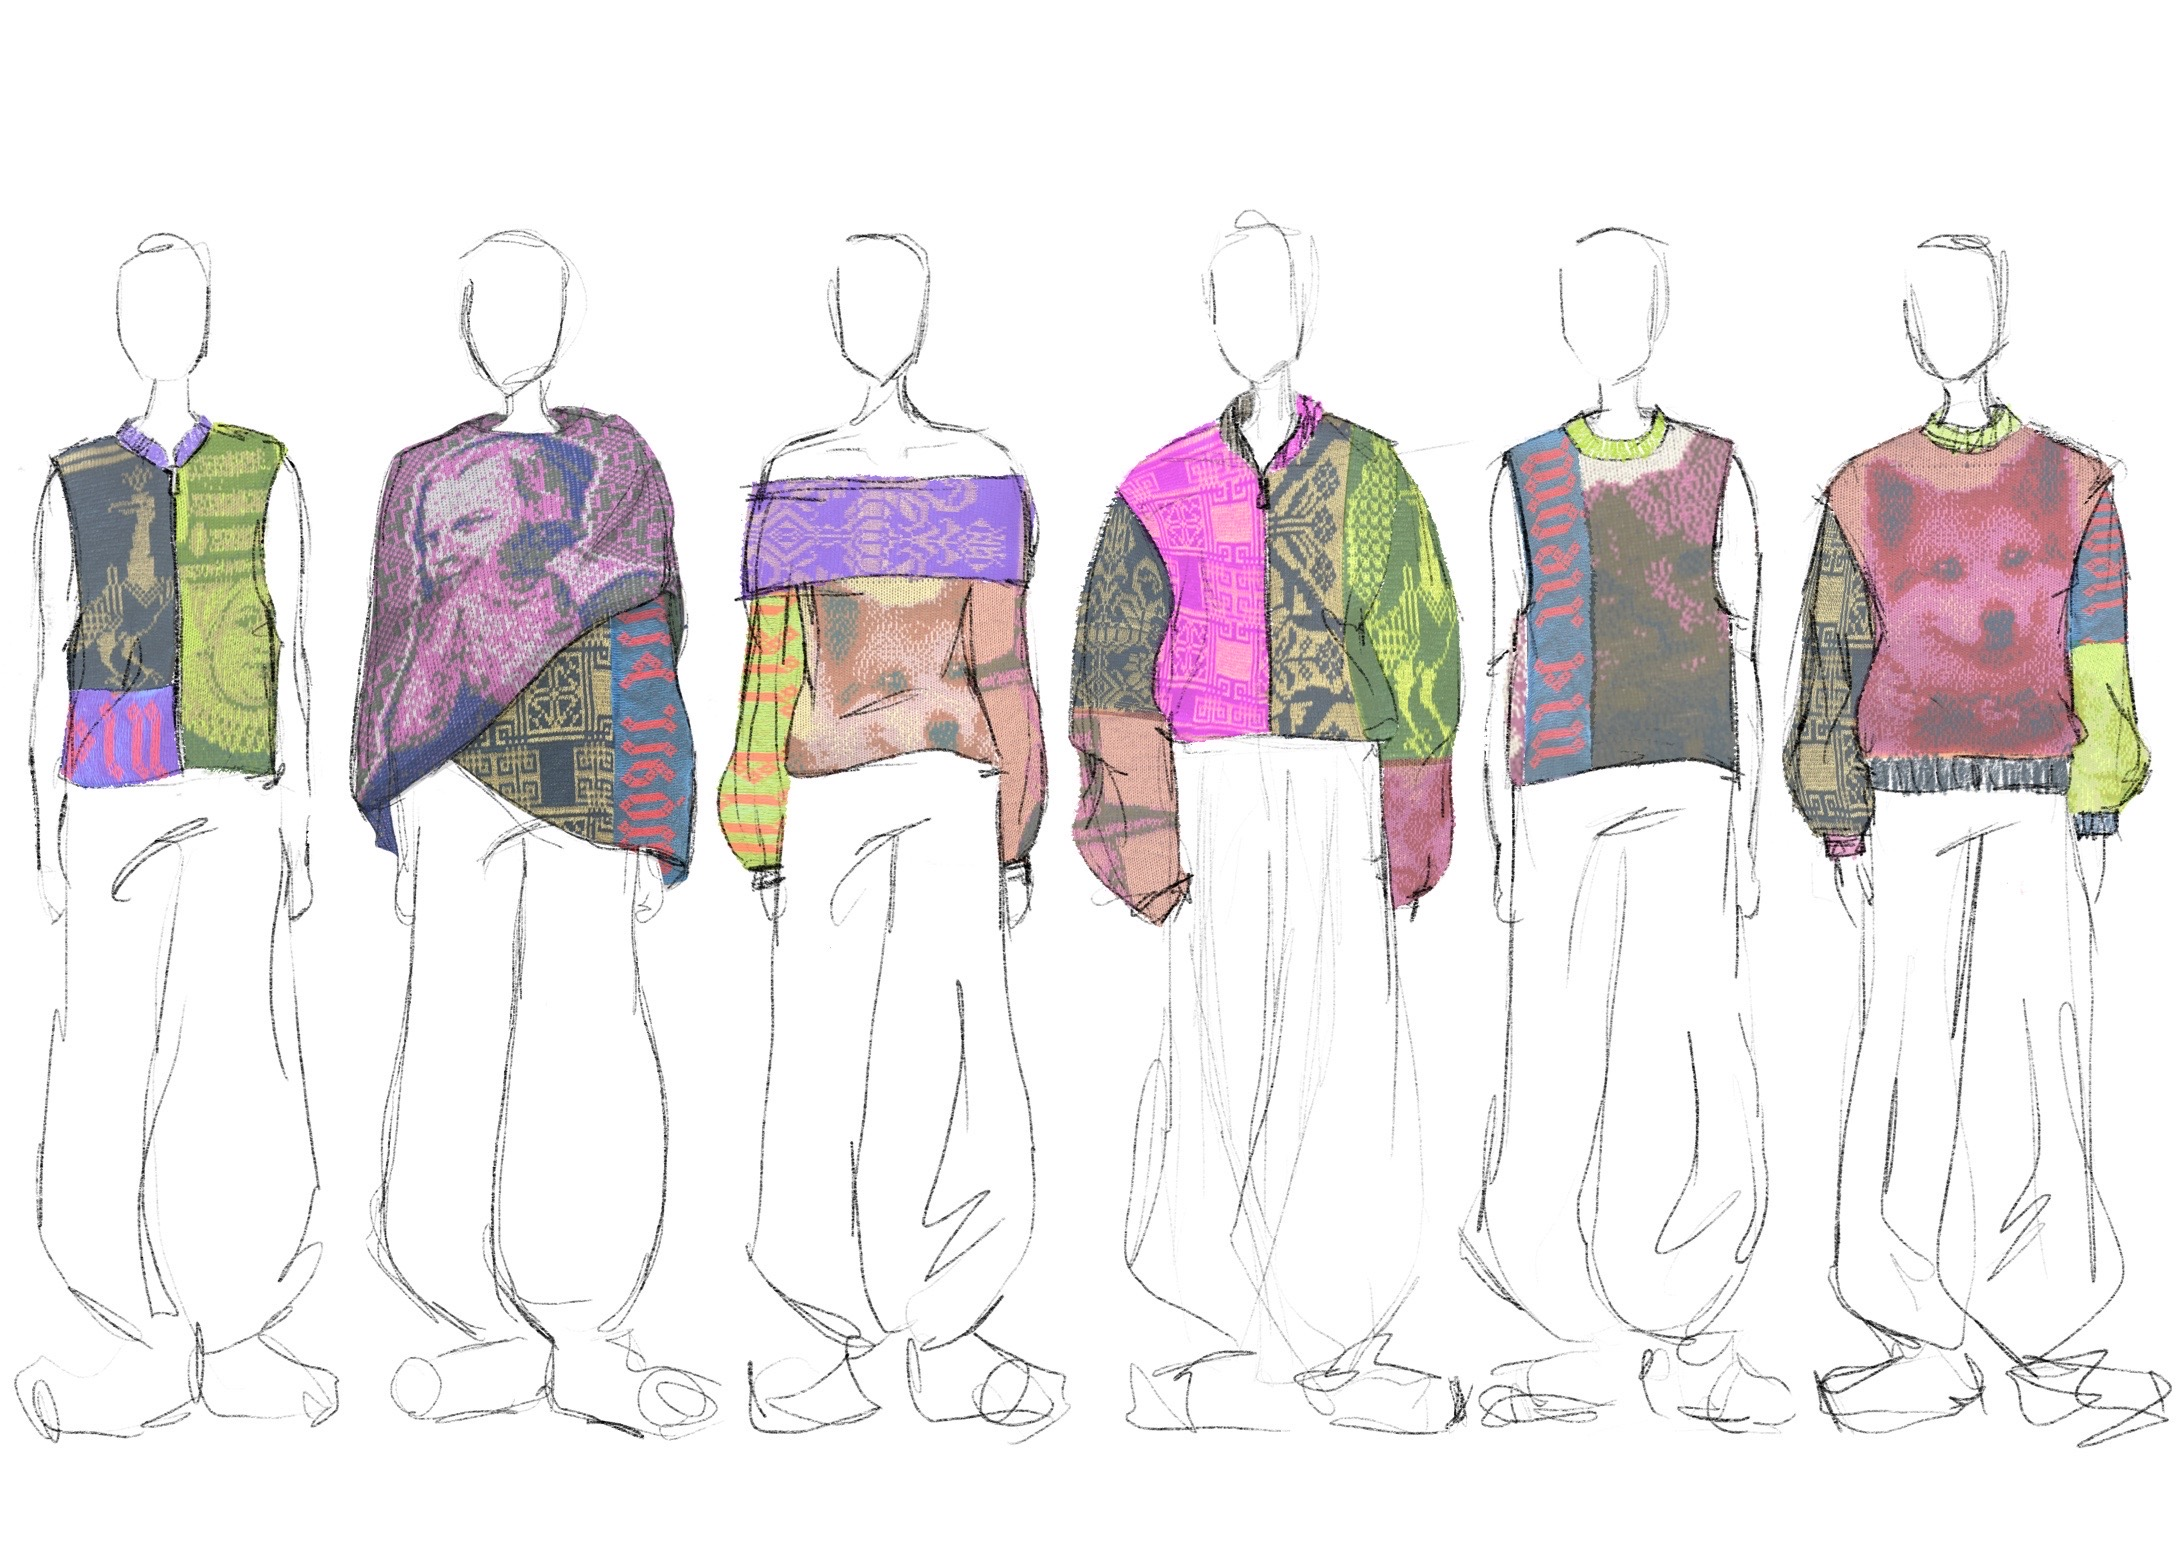
\includegraphics[width=\textwidth, trim=0 0 0 180pt, clip]{include/gisa.JPG}
    \end{frame}

    {
        \usebackgroundtemplate{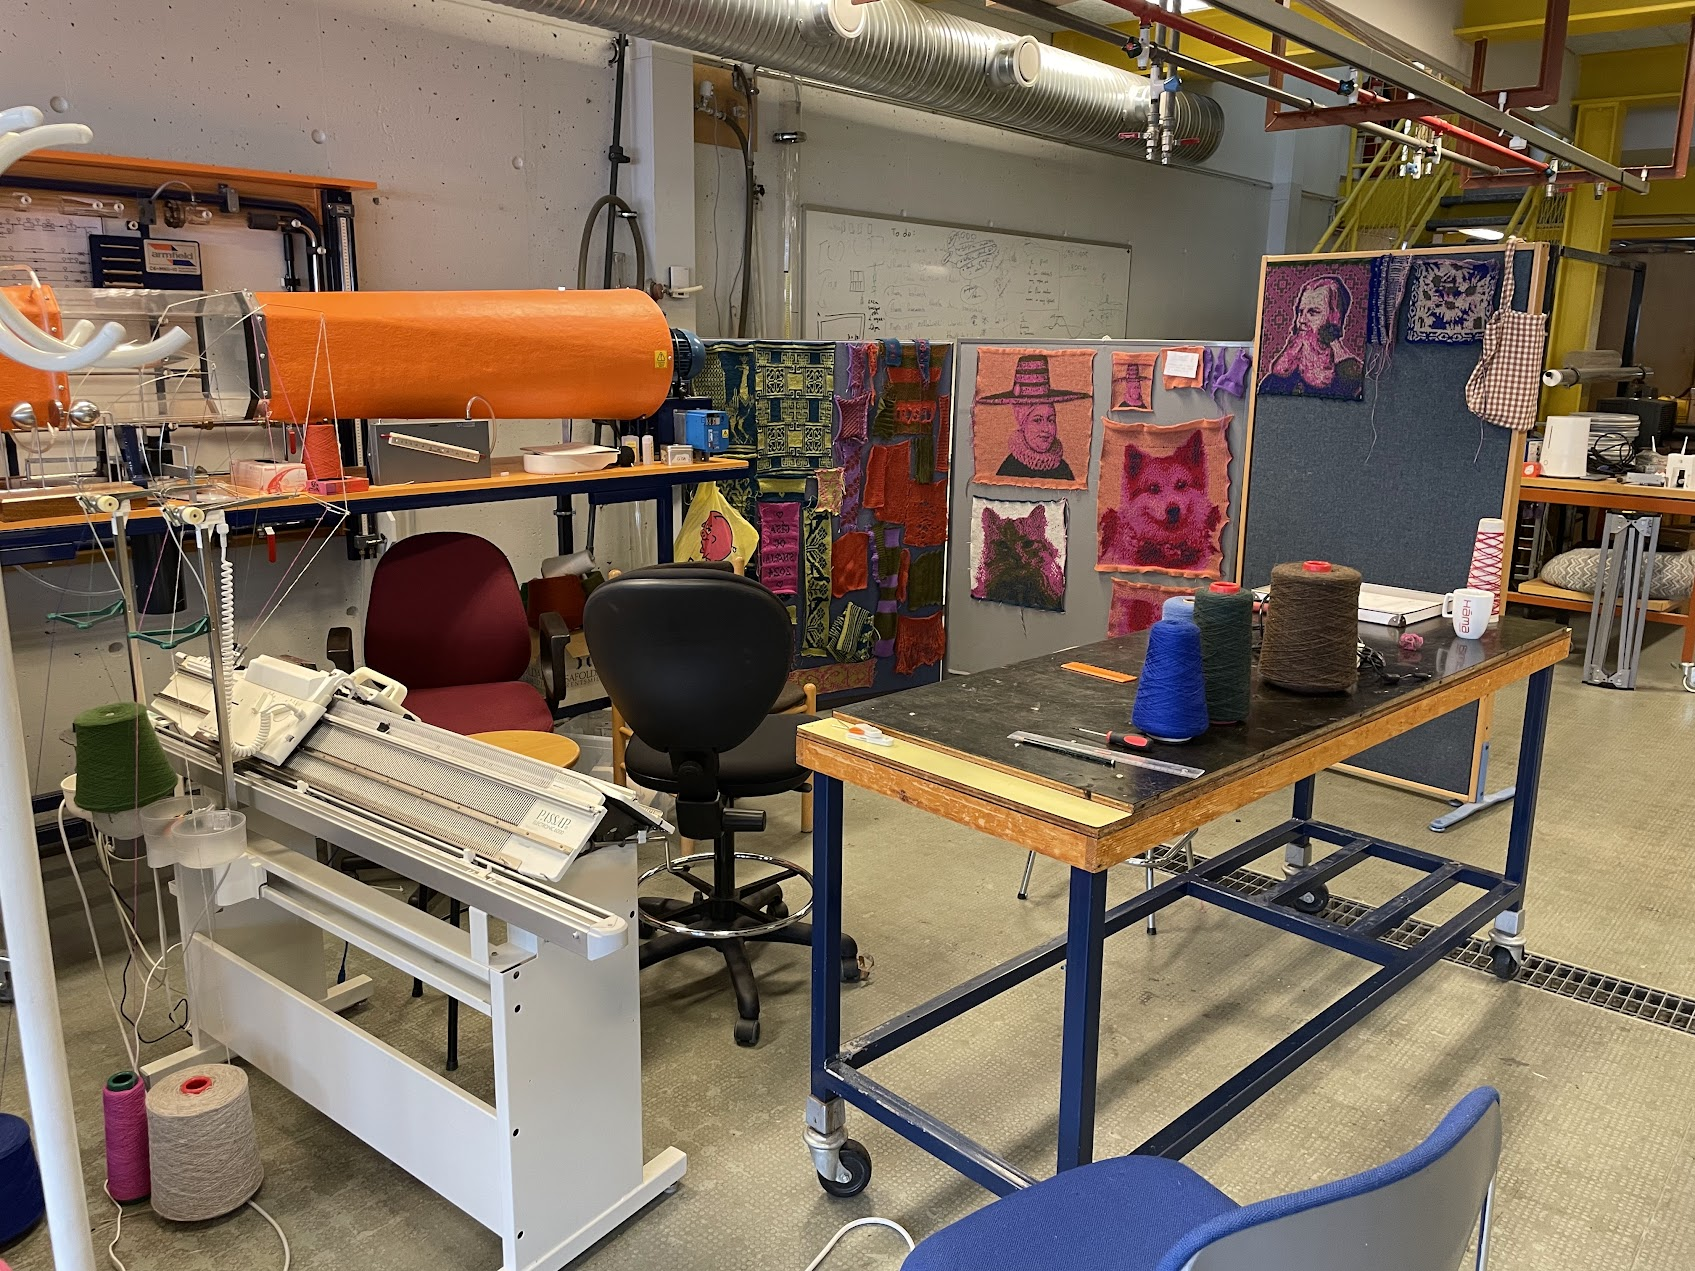
\includegraphics[width=\paperwidth]{include/workshop.jpg}}
        \begin{frame}
            \frametitle{Get in Touch}
            \vspace{2cm}
            \begin{columns}
                \begin{column}{0.4\textwidth}
                \end{column}
                \begin{column}{0.6\textwidth}
                    
\begin{tikzpicture}
                        \node[fill=white, fill opacity=0.8, text opacity=1, inner sep=5mm] (box) {%
                            \begin{minipage}{\textwidth}
                                \textbf{Websites:}

                                \vspace{0.5cm}

                                \begin{itemize}
                                    \item \url{https://github.com/HiDefTextiles/}
                                    \item \url{https://instagram.com/HiDefTextiles/}
                                \end{itemize}

                                \vspace{0.5cm}

                                \textbf{E-mail:} \href{mailto:helgaingim@hi.is}{helgaingim@hi.is}
                            \end{minipage}
                        };
                    \end{tikzpicture}
                \end{column}
            \end{columns}
        \end{frame}
    }

    \begin{frame}[allowframebreaks]{Stitch Pattern to Machine Commands}
        \begin{exampleblock}{Knitting One Row: Translation Function}
            \centering
            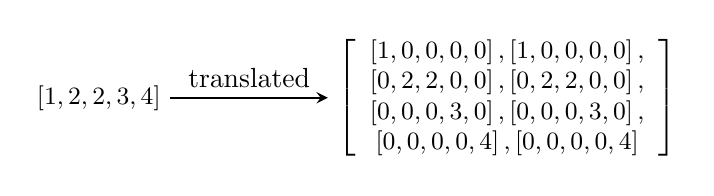
\begin{tikzpicture}[
                node distance=3cm and 2cm,
                arrow/.style={-stealth, thick},
                textstyle/.style={font=\small}
            ]
                % Pattern source node
                \node[textstyle] (pattern) {\( [1, 2, 2, 3, 4] \)};

                % Translated output node
                \node[textstyle, right=of pattern] (output) {\(
                \left[\begin{array}{c}
                          \left[1, 0, 0, 0, 0\right], \left[1, 0, 0, 0, 0\right], \\
                          \left[0, 2, 2, 0, 0\right], \left[0, 2, 2, 0, 0\right], \\
                          \left[0, 0, 0, 3, 0\right], \left[0, 0, 0, 3, 0\right], \\
                          \left[0, 0, 0, 0, 4\right], \left[0, 0, 0, 0, 4\right]
                \end{array}\right]
                \)};

                % Arrow and label
                \draw[arrow] (pattern.east) -- node[above] {translated} (output.west);
            \end{tikzpicture}
        \end{exampleblock}
        \vspace{1em}
        \textbf{Explanation:}
        \begin{itemize}
            \item Numbers \(1, 2, 3, 4\) specify the active color for knitting (max 4 supported).
            \item A \(0\) indicates a passive needle position (stitch not knitted in that pass).
            \item Each row requires 8 passes: one round trip for each color.
        \end{itemize}
        \framebreak
        \begin{figure}
            \centering
            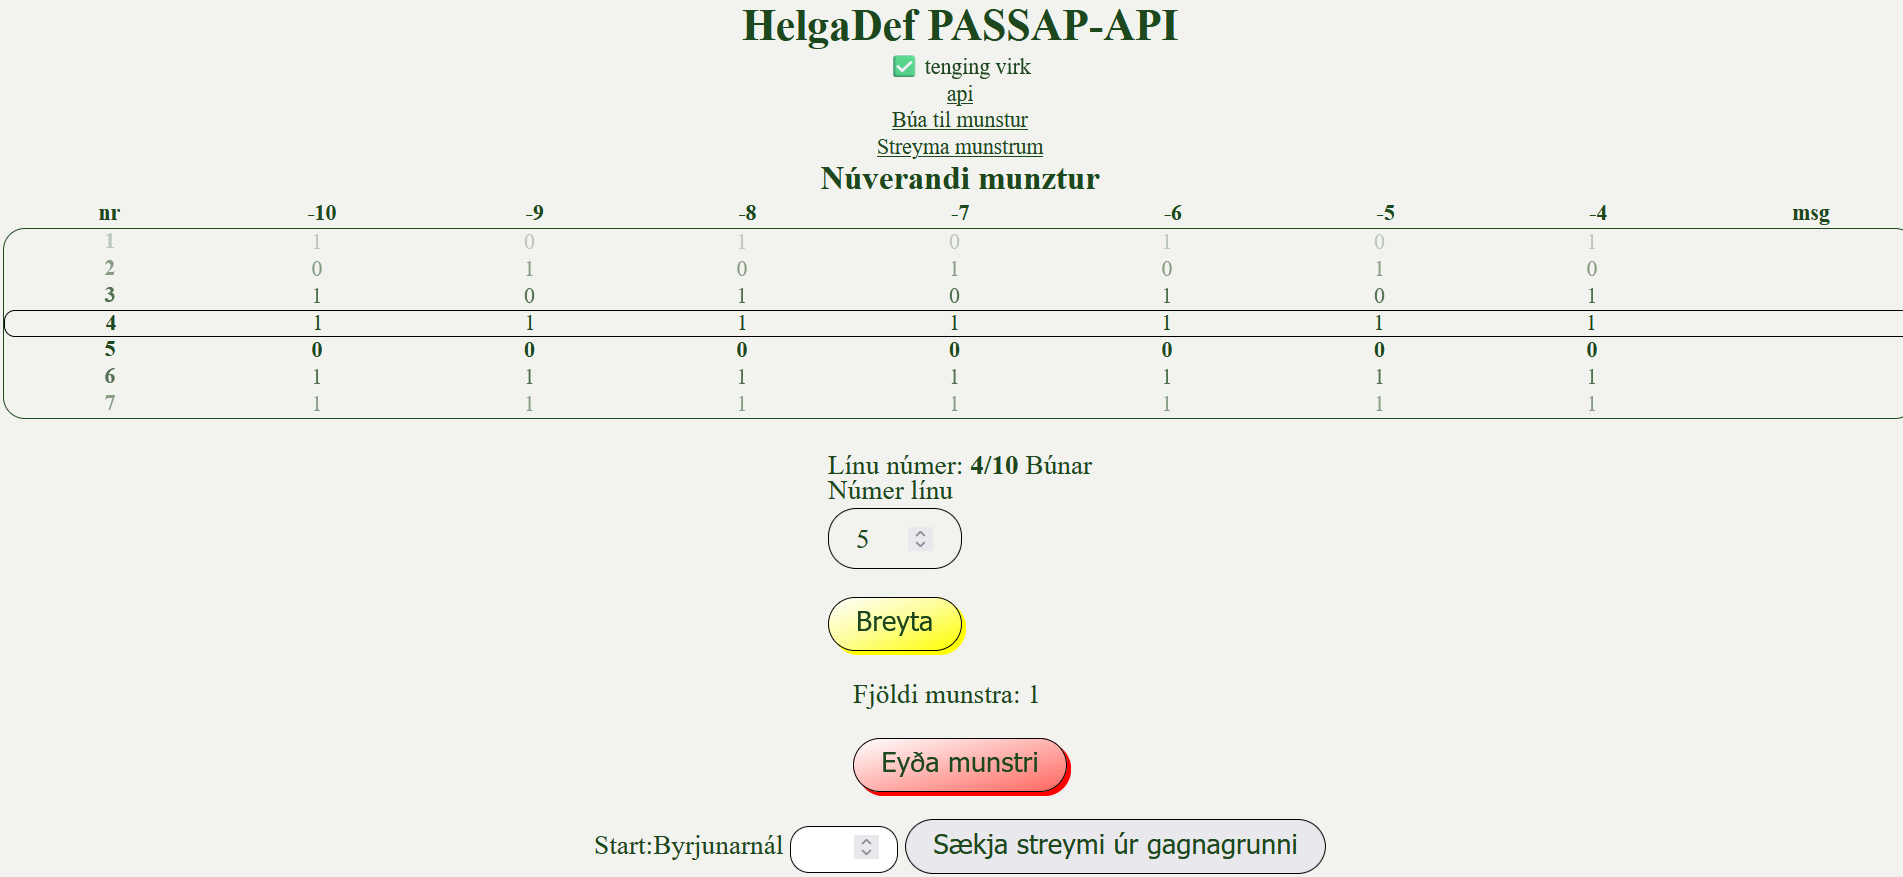
\includegraphics[width=.9\linewidth]{include/passapiscreen.png}
            \caption{Administrator interface of the controller}
        \end{figure}
    \end{frame}

    \begin{frame}{Motor Circuit Integration}
        \begin{columns}
            \begin{column}{0.5\textwidth}
                \begin{figure}
                    \centering
                    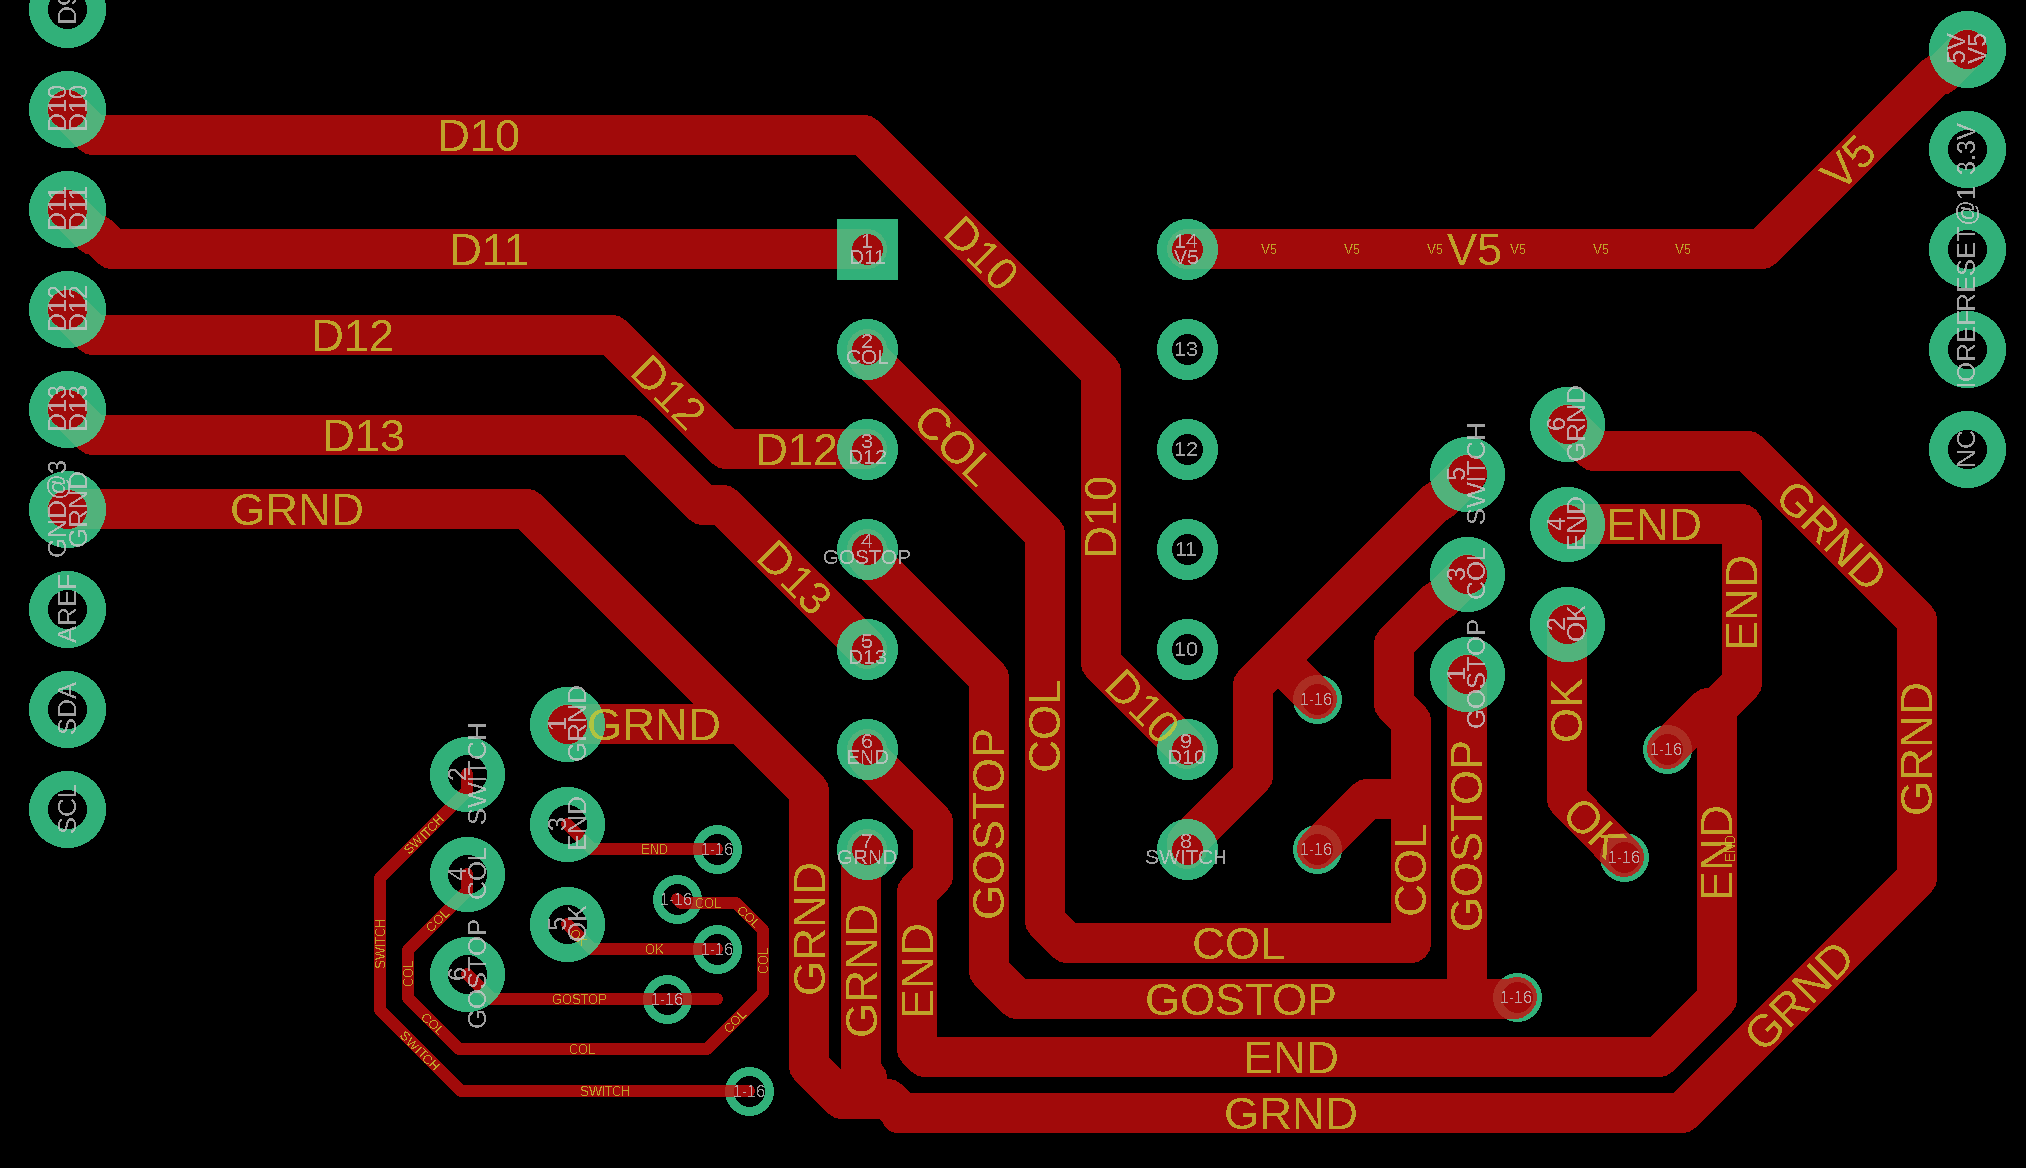
\includegraphics[width=0.9\linewidth]{include/PASSAPMOTOR.png}
                    \caption{Circuit diagram connecting an \textit{Arduino} to a 7407N chip, which interfaces with a 6-pin RJ12 connector to control the motor.}
                \end{figure}
            \end{column}
            \begin{column}{0.5\textwidth}
                \begin{figure}
                    \centering
                    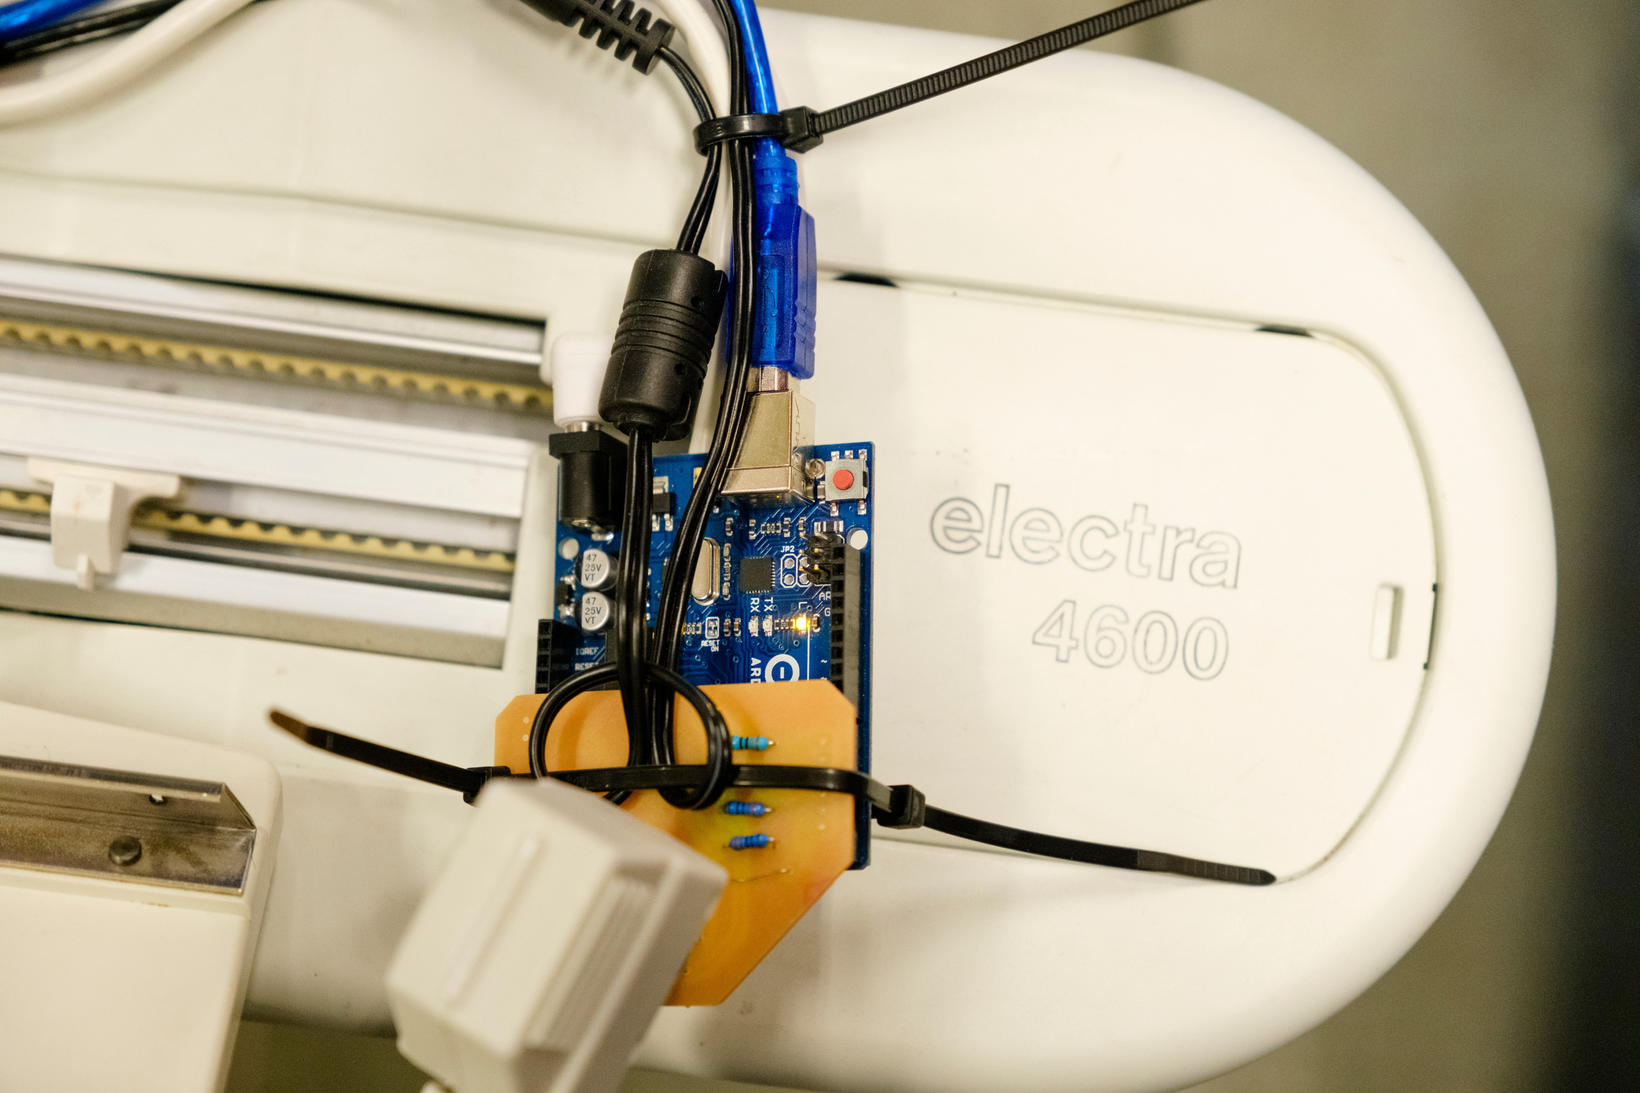
\includegraphics[width=0.9\linewidth]{include/electra4600.jpg}
                    \caption{The physical circuit implementation on the knitting machine.}
                \end{figure}
            \end{column}
        \end{columns}
    \end{frame}

    \begin{frame}{Instagram Reels \texttt{@hideftextiles}}
    \centering
        \href{https://www.instagram.com/p/C7kbxeFIKz1/}{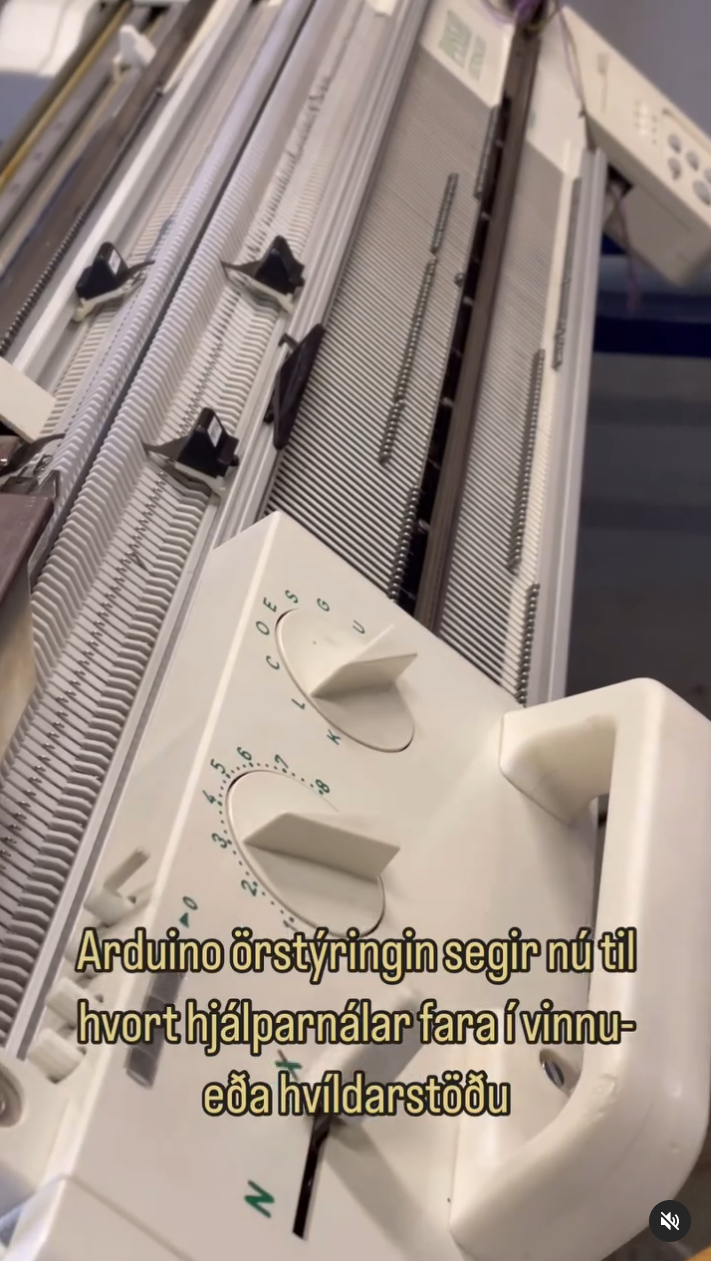
\includegraphics[height=0.8\textheight]{include/C7kbxeFIKz1.png}}
        \href{https://www.instagram.com/p/C9Cf8FFgDZZ}{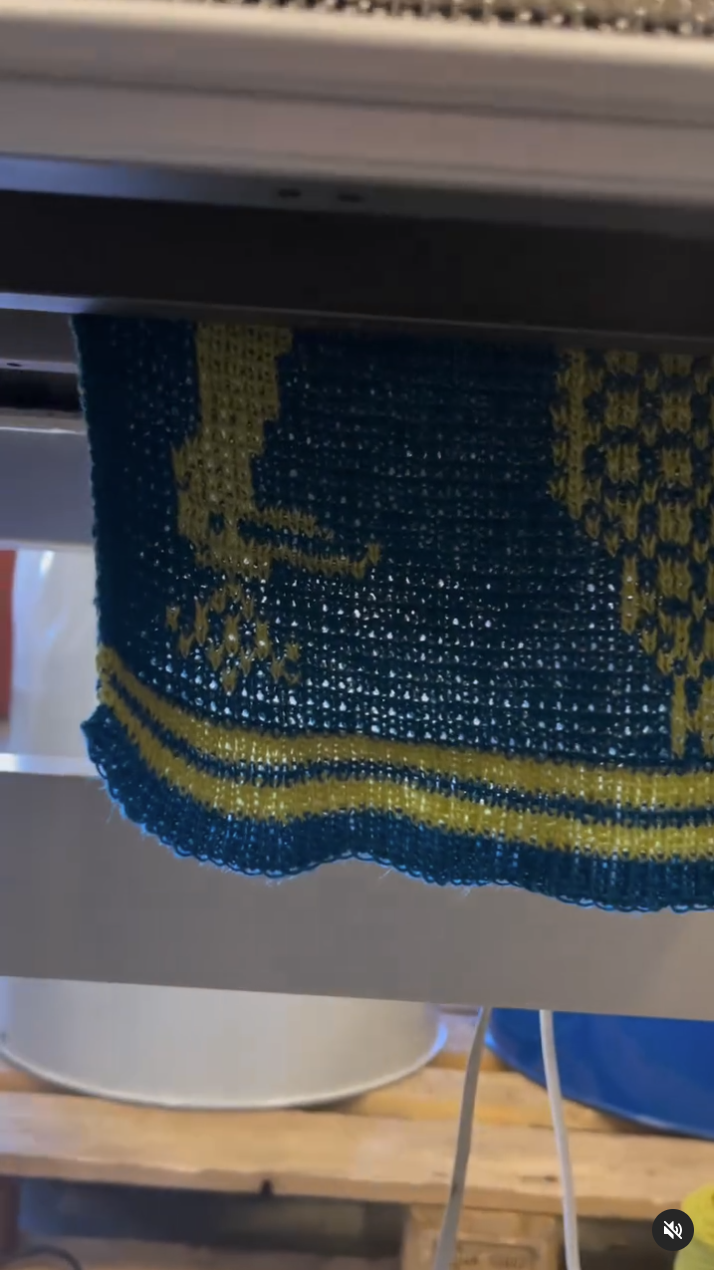
\includegraphics[height=0.8\textheight]{include/C9Cf8FFgDZZ.png}}
        \href{https://www.instagram.com/p/C766unfoZAJ/}{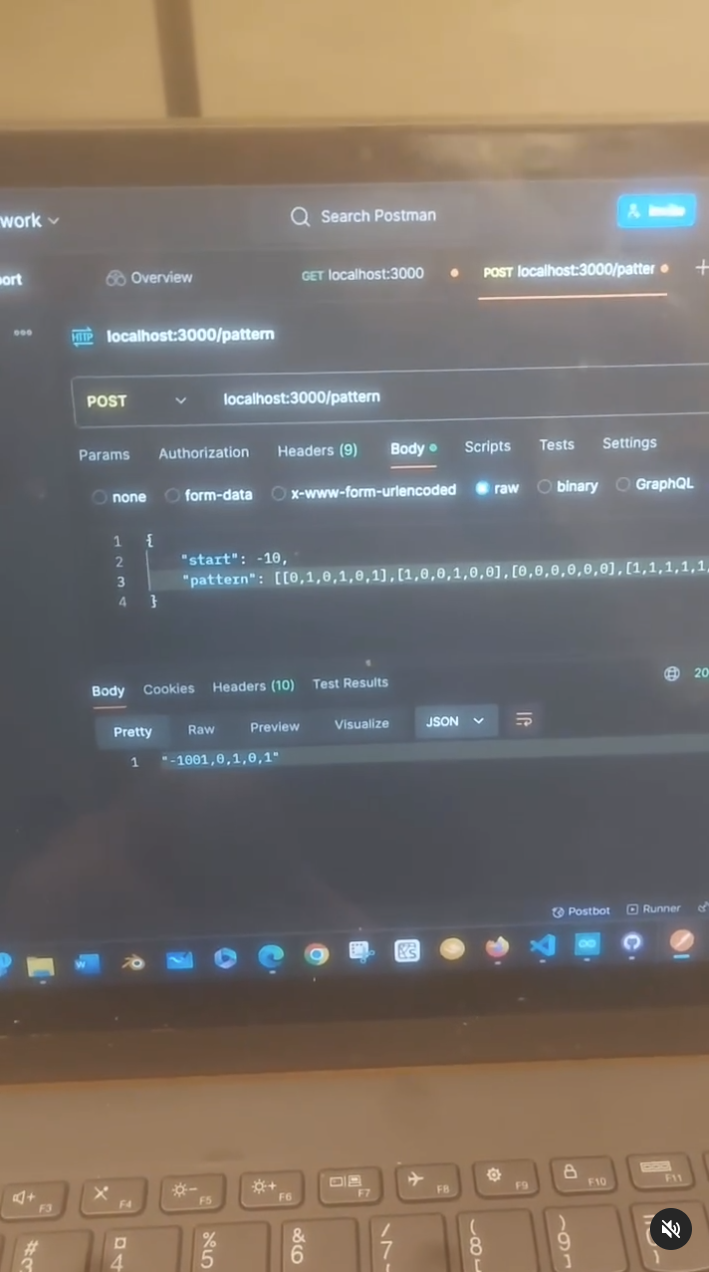
\includegraphics[height=0.8\textheight]{include/C766unfoZAJ.png}}
        
\includegraphics[width=0.2\linewidth]{include/hideftextiles_qr.png}
    \end{frame}

\end{document}
